\documentclass[11pt]{article}
\usepackage[preprint]{acl}
\usepackage{times}\renewcommand{\ttdefault}{lmtt}
\usepackage[T1]{fontenc}\usepackage[utf8]{inputenc}
\usepackage{microtype,amsmath,amssymb,booktabs,graphicx,url}
\extrafloats{100}
\title{Attention and Personal Calibration for VitalDB Blood-Pressure Estimation: Bad-Blood v2}
\author{Bad-Blood Project\\Research and Engineering Report}
\begin{document}\maketitle
\begin{abstract}
We evaluate lightweight attention interventions on the actual high-resolution
Bad-Blood CNN and early personal calibration for later contemporaneous blood-
pressure estimation. Waveform models receive ten-second ECG/PPG windows and output
scalar SBP/DBP. The controlled population comparison excludes previously
explored personal patients and retrains the unchanged baseline. A separate
six-patient chronological pilot evaluates sparse ABP-reference calibration,
with adaptation settings chosen on four different patients. Results below
are computed from completed, hash-verified experiments, not simulations of
model accuracy. Sparse references are simulated from real invasive labels;
they are not actual cuff events.
The prospective four-model validation comparison retains the unchanged CNN, whose primary-test patient-macro SBP/DBP MAE, averaged across seeds 42/43/44, is 12.59/8.36 mmHg. Separately, SE-last has primary-test SBP/DBP MAE 12.386/8.002 mmHg; SE-minus-CNN changes are SBP -0.20 [-0.48, +0.07]; DBP -0.36 [-0.53, -0.18] mmHg (descriptive paired 95\% patient intervals). Across the six required three-seed models, the lowest observed primary-test MAEs are SBP 12.386 mmHg for SE-last and DBP 8.002 mmHg for SE-last. These observed test comparisons do not change validation-based selection. With ten simulated personal references, three-seed mean patient-macro population and full-adaptation MAE are 12.73/7.80 and 9.24/4.66 mmHg; bias correction gives 9.02/4.84, and reference mean gives 9.01/4.04. Paired patient intervals and all individual cases qualify these descriptive comparisons.

\end{abstract}
\section{Research questions and motivation}
The application is a population-trained estimator that can be calibrated to
one person and then use newly observed ECG/PPG to estimate their current
pressure. Track A asks whether attention improves the existing architecture
at matched training and data budgets. Track B asks how adaptation depth and
reference budget affect later error and how performance changes over time.
These hypotheses do not assume that larger models or more adaptation improve
every patient. Later ECG/PPG is a legitimate input; later BP is evaluator-only.
The task is not open-loop future-waveform prediction.

\section{Related work}
SE, ECA and CBAM motivate feature-channel and temporal gates
\citep{hu2018se,wang2020eca,woo2018cbam}. Learned feature channels are not
individual sensors after convolutional mixing. Physiological hybrids offer
relevant precedents but differ in calibration, scale and splitting; their
reported numbers are not interchangeable benchmarks. One-reference conditioning
\citep{schlesinger2020} and restricted-layer transfer \citep{leitner2022} motivate
the personal comparison. Shuffled within-patient evaluation does not establish
durability. Real longer-term evidence is sensor- and model-specific
\citep{yavarimanesh2022}, while strong reference-only comparators are essential
\citep{mieloszyk2022}. The two accompanying ACL literature reviews document
paper-level definitions, reported metrics, provenance and limitations.

\section{Data and provenance audit}
Official VitalDB-specific PulseDB subsets provide the population data
\citep{wang2023pulsedb}. Source suffix 1 identifies VitalDB, not a visit. All 31
case-to-subject links in complete local individual files were checked against
public VitalDB metadata. The population subsets contain no timestamps or case
IDs; temporal evaluation instead uses individual files with original T and
CaseID. Raw ABP, derived labels and QC fields never enter the inference inputs.

Excluding all 31 historically explored patients leaves 1,085 training patients
(390,600 windows), 192 validation patients (69,120), 141 primary-test patients
(56,400), and 116 stress-test patients (666). Original V1 scores are historical
and are not treated as the new baseline. Previous project work inspected the
test cohort, so this is a controlled rerun rather than untouched external
validation. All new population weights exclude the personal patients.

Thirty complete individual files contain 30 patients, 31 cases and 15,486
windows. One truncated and one absent file are excluded; two patients have
only two isolated windows. A multi-case patient is not used for the main
within-case pilot. Availability-only allocation gives four development and
six final patients. One initially selected patient lacked ten spaced early
references and was replaced before training, with the complete audit trail
retained. Final patients provide 4,284 later queries; development provides 1,855.
Two query-to-query timestamp pairs overlap by 8 ms upstream; no support/query
boundary is crossed. No local actual cuff/NIBP events or dated repeat visits
support clinical cuff or cross-visit claims.

\section{Methods and controlled design}
\subsection{Architecture and population fitting}
The V1 source last changed at commit \texttt{1f33cdc}; the research base is
\texttt{7553248}. The exact 37,666-parameter BPNet(pool=1) has a 2-to-8 stem
(kernel 7, stride 2), residual blocks 8-to-16-to-32-to-48 (kernels 7 and 5),
BatchNorm/SiLU, global mean pooling and a 48-to-32-to-2 head with dropout 0.15.
Residual feature lengths are 313, 157 and 79.
SE-last uses a 48-to-6-to-48 MLP; temporal attention uses mean/max channel
pooling and a seven-tap convolution; CBAM1D applies channel then temporal
gates. A 630-parameter additive pooled-context control matches SE capacity.
SE-all tests placement. ECG-only/PPG-only ablations zero the absent channel.
ECA is explicitly supplementary. All parameters and state keys are tested
against the original implementation, rather than approximating the backbone.
Figure~\ref{fig:architecture} shows the shared backbone and intervention point.
\begin{figure*}[t]\centering
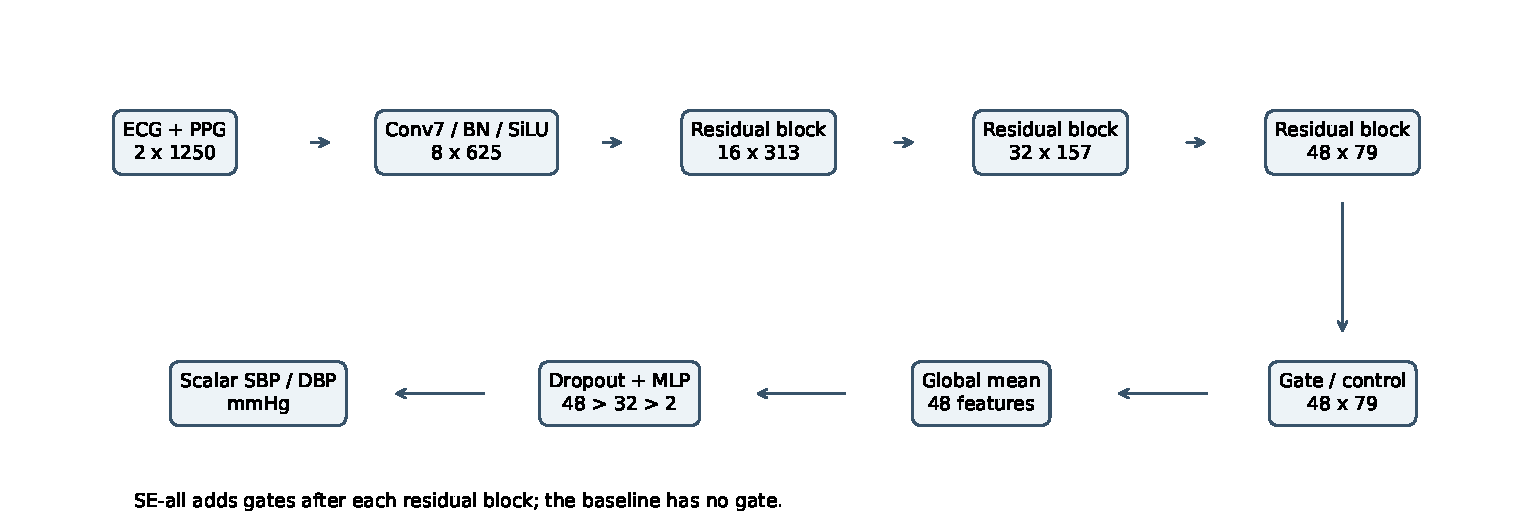
\includegraphics[width=\textwidth]{figures/architecture.pdf}
\caption{The unchanged high-resolution backbone and final-block intervention.
Shapes omit batch size. Inputs are observed, contemporaneous ECG/PPG;
outputs are scalar pressures.}\label{fig:architecture}\end{figure*}

Inputs use provided filtered fields with per-window/channel min--max scaling.
For observed window $X$, the physical-unit prediction is
\begin{equation}
g_\theta(X)=\mu_{\rm tr}+\sigma_{\rm tr}\odot f_\theta(N(X)),
\end{equation}
where $N$ scales each input channel within that window. Labels use
training-only centering/scaling: $\mu_{\rm tr}=(115.418,62.928)$ and
$\sigma_{\rm tr}=(18.942,12.083)$ mmHg, in SBP/DBP order. All fits use normalized MSE,
AdamW (learning rate 0.001, weight decay 0.001), batch size 256, noise SD 0.003,
gradient clipping at norm 5, maximum 40 epochs, and patience 8. A factor-0.5,
patience-3 plateau scheduler and best-checkpoint selection use mean validation
patient-macro SBP/DBP MAE. Seeds 42/43/44 are matched for principal comparisons;
modality ablations use 42 only. Source,
split, config and checkpoint hashes accompany every run. Epoch-boundary
resume restores optimizer, scheduler and RNG states.

\subsection{Personal calibration}
Each case's first 20\% of elapsed span defines the support period; query windows
start after a 10-second boundary guard. Gaps are retained. From a greedy pool
with starts at least 60 seconds apart, ten approximately evenly spaced references
are selected; budgets 1, 2, 3, 5 and 10 use nested prefixes. Queries stay identical
across budgets. Labels are invasive-ABP-derived sparse references, not cuff
measurements or independent evidence merely because they are spaced.

New unchanged baseline checkpoints initialize all strategies at matched seeds.
Comparisons are no adaptation, additive residual bias, shrinkage affine
($K\geq3$), head-only, last-block-plus-head, full-model, last-reference and
calibration-mean controls. The last two do not need ECG/PPG at prediction.
Head, last-block and full train 1,634, 25,730 and 37,666 parameters respectively.
BN running state and dropout remain fixed. Neural learning rates 0.0001/0.001
and steps 20/100, and affine penalties 1/10/100, are selected only on the four
development patients averaged across seeds. No final patient's later labels
control adaptation stopping, parameter selection or normalization.
Bias calibration adds the support mean residual,
\begin{equation}
\delta_i=\frac{1}{K}\sum_{j=1}^{K}\bigl(y_{ij}-g_\theta(X_{ij})\bigr),
\end{equation}
to each later prediction. For each pressure separately, affine calibration
fits $a z_j+b$ to standardized support labels $u_j$ by minimizing
$\sum_j(u_j-a z_j-b)^2+\lambda(a-1)^2$; the intercept is unpenalized.
Last-reference and reference-mean controls predict the corresponding scalar
support pressure without using later waveforms. Neural adaptation minimizes
the same standardized two-output MSE on all $K$ support windows for the
development-selected number of updates; it never monitors later BP loss.
The nested chronological prefixes vary both reference count and reference
recency. Budget curves therefore describe this acquisition policy, not pure
sample complexity with reference age held constant.
Figure~\ref{fig:personal_task} separates calibration, later inference and evaluation.
\begin{figure*}[t]\centering
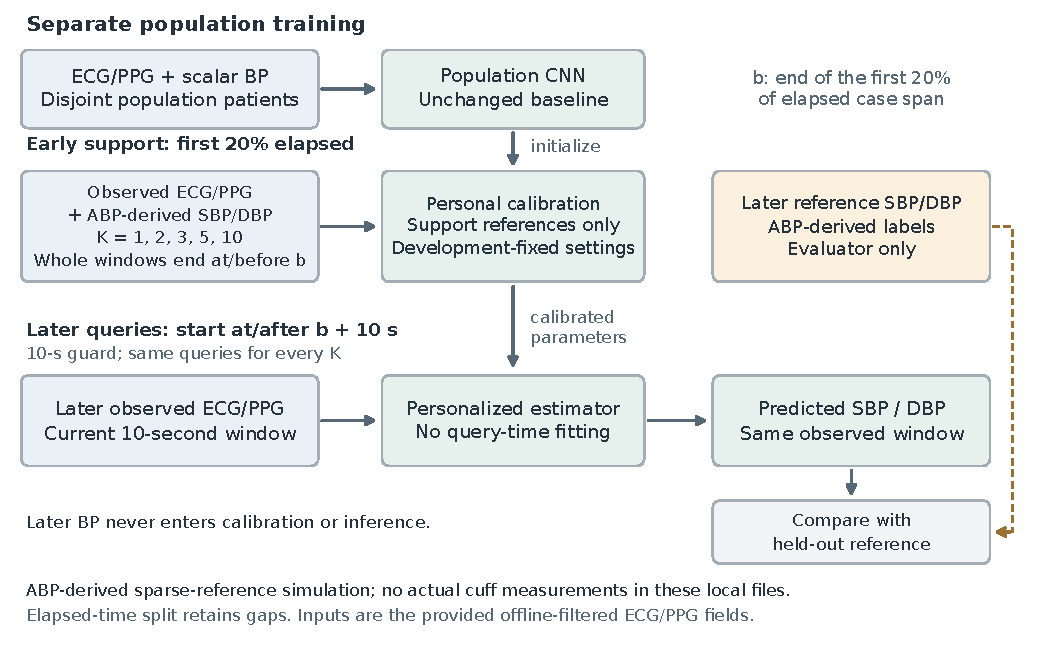
\includegraphics[width=\textwidth]{figures/personal_task.pdf}
\caption{Personal calibration and later contemporaneous inference. Only early
invasive-ABP-derived scalar references fit the personal parameters. Later
observed ECG/PPG enters the estimator; later blood-pressure labels enter only
the evaluator. The 20\% split uses elapsed case span and preserves recording
gaps.}\label{fig:personal_task}\end{figure*}

\subsection{Evaluation and uncertainty}
MAE/RMSE, bias, sample error SD, median and 90th/95th error quantiles,
within-5/10/15-mmHg fractions, correlation and $R^2$ are saved separately
for SBP and DBP. Patient-macro metrics weight people equally; pooled metrics
weight windows equally. Paired changes average matched seeds within patient,
then resample patients 2,000 times for descriptive 95\% intervals. Seed SD and
patient uncertainty are separate. Reference-only predictors have identical
predictions across seeds by construction; zero seed SD does not imply zero
patient uncertainty or three independent replications. Counts of patients
with lower error describe its sign, not a minimum practically important change.
Pressure strata and all patient failures
remain visible. Repeated-measurement Bland--Altman summaries decompose
between/within-person error; serial correlation remains a limitation.
Drift uses time from the actual last support reference, not silently the 20\%
boundary. Empty bins are unavailable, not zero error. The saved secondary
boundary-relative analysis uses a distinct label.
For one pressure and errors $e_{ij}=\hat y_{ij}-y_{ij}$, the primary
patient-macro definitions are
\begin{align}
{\rm MAE}_{\rm macro}&=\frac{1}{P}\sum_i\frac{1}{n_i}\sum_j|e_{ij}|,\\
{\rm RMSE}_{\rm macro}&=\frac{1}{P}\sum_i\sqrt{\frac{1}{n_i}\sum_j e_{ij}^2}.
\end{align}
Pooled RMSE instead takes one square root after averaging all window errors.
Error SD uses denominator $N-1$; threshold fractions include equality.
Correlations and $R^2$ with zero required variance are undefined, not zero;
macro summaries retain the number of patients for whom each metric exists.

\section{Results}
Figure~\ref{fig:attention_results} summarizes population errors.
Figures~\ref{fig:personal_budget} and~\ref{fig:personal_drift} show the
personal-reference budget and elapsed-time analyses; the paired time-bin
effects are in Figure~\ref{fig:drift_gain}. Individual paired changes are in
Figure~\ref{fig:patient_changes}, with chronological examples in
Figure~\ref{fig:temporal_examples} and observed input signals in
Figure~\ref{fig:observed_waveforms}. Figure~\ref{fig:repeated_bland_altman}
shows descriptive agreement. Appendix~\ref{sec:complete} provides complete
paired, pressure-range, budget and patient-level tables.
The unchanged CNN ranks first on validation among all six required three-seed architectures, including capacity and placement controls. Its primary-test patient-macro SBP/DBP MAE, averaged across seeds 42/43/44, is 12.59/8.36 mmHg. The four-model attention ranking is reported separately below; neither ranking uses test accuracy. Unless explicitly labeled seed 42, principal-model results average three separately evaluated checkpoints, not one seed-42 run or an ensemble of predictions.

At K=10, Bias changes SBP/DBP MAE by -3.71/-2.96 mmHg; 4/6 patients improve in SBP and 4/6 in DBP.

At K=10, Head changes SBP/DBP MAE by -2.27/-2.84 mmHg; 4/6 patients improve in SBP and 5/6 in DBP.

At K=10, Last block changes SBP/DBP MAE by -3.46/-3.05 mmHg; 5/6 patients improve in SBP and 5/6 in DBP.

At K=10, Full changes SBP/DBP MAE by -3.49/-3.14 mmHg; 5/6 patients improve in SBP and 5/6 in DBP.



\paragraph{Validation choices.}

Within the four-model attention comparison (CNN, SE-last, Temporal and CBAM1D), validation selects CNN (mean SBP/DBP patient-macro MAE 10.37 mmHg). The separate required three-seed comparison, which also includes Additive and SE-all, selects CNN (10.37 mmHg). The choices coincide. Both choices use validation only; capacity, placement and modality contrasts retain their distinct roles, and optional ECA is supplementary. Table~\ref{tab:attention_validation} separates validation SBP/DBP errors from the combined selection scores. A run is one architecture at one seed: its checkpoint is selected using that run's validation history. An architecture is ranked by the mean validation score of its three selected runs. Reported three-seed metrics average separately evaluated checkpoints, not predictions in an ensemble; a seed-42 score is one run, not the three-seed mean.

\begin{table*}[t]\centering\small\setlength{\tabcolsep}{5pt}
\begin{tabular}{lrrrrrr}\toprule
Model & SBP mean & DBP mean & $Q_{42}$ & $Q_{43}$ & $Q_{44}$ & $\overline{Q}$\\\midrule
CNN & 12.410 & 8.332 & 10.375 & 10.393 & 10.345 & 10.371\\
SE-last & 12.515 & 8.264 & 10.291 & 10.457 & 10.421 & 10.390\\
Temporal & 12.487 & 8.323 & 10.299 & 10.466 & 10.450 & 10.405\\
CBAM1D & 12.521 & 8.294 & 10.379 & 10.383 & 10.461 & 10.408\\
\midrule
Additive & 12.442 & 8.340 & 10.400 & 10.366 & 10.407 & 10.391\\
SE-all & 12.466 & 8.323 & 10.412 & 10.454 & 10.317 & 10.394\\
\bottomrule\end{tabular}
\caption{Validation patient-macro MAE (mmHg), not primary-test error. Every run uses its own validation-selected checkpoint. SBP and DBP means average seeds 42/43/44; $Q_s=({\rm MAE}_{s,\rm SBP}+{\rm MAE}_{s,\rm DBP})/2$ is one seed's score, and $\overline{Q}=(Q_{42}+Q_{43}+Q_{44})/3$ ranks architectures. The first four rows form the attention comparison; Additive and SE-all are capacity and placement controls in the separate six-model ranking. Values are rounded to three decimals for display only; selection uses unrounded values.}\label{tab:attention_validation}\end{table*}

\paragraph{Attention effects and heterogeneity.}

The following are primary-test MAE changes with descriptive paired 95\% patient intervals, in mmHg, relative to the same-seed CNN. Negative values reduce error. SBP and DBP remain separate rather than being replaced by the selection scalar.

SE-last: SBP -0.20 [-0.48, +0.07]; DBP -0.36 [-0.53, -0.18]. SBP/DBP macro MAE is lower in 3/3 and 3/3 matched seeds; seed-averaged patient MAE is lower for 81/141 and 96/141 patients. The two targets do not show a uniform directional advantage with both intervals on one side of zero; this is not evidence of equivalence.

Temporal: SBP -0.01 [-0.19, +0.19]; DBP -0.06 [-0.18, +0.07]. SBP/DBP macro MAE is lower in 1/3 and 3/3 matched seeds; seed-averaged patient MAE is lower for 71/141 and 76/141 patients. The two targets do not show a uniform directional advantage with both intervals on one side of zero; this is not evidence of equivalence.

CBAM1D: SBP -0.17 [-0.47, +0.13]; DBP -0.25 [-0.43, -0.08]. SBP/DBP macro MAE is lower in 3/3 and 3/3 matched seeds; seed-averaged patient MAE is lower for 72/141 and 86/141 patients. The two targets do not show a uniform directional advantage with both intervals on one side of zero; this is not evidence of equivalence.

Intervals spanning zero do not establish equivalence, while intervals excluding zero remain unadjusted for the multiple architecture/endpoint contrasts. These intervals condition on the fitted seeds: the separate seed counts and SDs describe training variability. An average gain is not a guarantee for every patient or pressure range, and no minimum clinically useful effect was prespecified.

\paragraph{Architectural controls.}

SE-last minus Additive changes MAE by SBP -0.27 [-0.50, -0.05]; DBP -0.17 [-0.29, -0.06]. Both descriptive MAE intervals favor SE-last over Additive under the fixed fitting settings. Both contain 38,296 parameters, so parameter count alone cannot distinguish these specified operators. This is not proof that all attention mechanisms or all optimizers would behave similarly.

SE-all minus SE-last gives SBP +0.11 [-0.14, +0.37]; DBP +0.23 [+0.05, +0.42]. The two targets do not show a uniform directional advantage with both intervals on one side of zero; this is not evidence of equivalence. SE-all inserts gates at three residual outputs and has 374 more parameters than SE-last; the contrast combines insertion depth with capacity, not a pure relocation. The direct CBAM1D-versus-SE and CBAM1D-versus-Temporal MAE/RMSE contrasts are tabulated below. CBAM1D also changes channel pooling from SE's average-only descriptor to shared average/max descriptors, so it is not a factorial test isolating the added temporal gate.

\paragraph{Observed-sensor ablations.}

The zero-channel models are retrained baselines, not missing-sensor tests of the trained two-sensor model. At seed 42, PPG-only primary-test patient-macro SBP/DBP MAE is 12.296/7.771 mmHg, versus 12.603/8.235 for CNN and 12.366/7.949 for SE-last. PPG-only has lower observed point errors on both endpoints than both comparators in this run. These matched-seed point estimates are single-run evidence, not a three-seed superiority claim. ECG only minus CNN MAE: SBP +1.71 [+0.84, +2.52]; DBP +0.87 [+0.19, +1.57]; PPG only minus CNN MAE: SBP -0.31 [-0.79, +0.20]; DBP -0.46 [-0.84, -0.07]. ECG only removes PPG, whereas PPG only removes ECG. Their patient intervals condition on seed 42 and cannot establish seed-robust sensor importance or an attention-by-modality interaction. Learned feature-channel gates do not themselves identify physiological sensor importance.

Accuracy gains must be weighed against the separately measured parameters and CPU/MPS latency; parameter overhead alone is not measured speed or evidence of native-device readiness.

\begin{table*}[t]\centering\scriptsize\setlength{\tabcolsep}{4pt}\renewcommand{\arraystretch}{1.15}
\begin{tabular}{lrrr}\toprule
Contrast (left minus right) & Seeds & SBP change [95\% CI] & DBP change [95\% CI]\\\midrule
\shortstack{SE-last minus Additive\\{capacity-matched operator}} & 3 & \shortstack{-0.27\\{[-0.50, -0.05]}} & \shortstack{-0.17\\{[-0.29, -0.06]}}\\
\shortstack{SE-all minus SE-last\\{insertion depth and capacity}} & 3 & \shortstack{+0.11\\{[-0.14, +0.37]}} & \shortstack{+0.23\\{[+0.05, +0.42]}}\\
\shortstack{CBAM1D minus SE-last\\{combined versus channel gate}} & 3 & \shortstack{+0.03\\{[-0.22, +0.28]}} & \shortstack{+0.11\\{[-0.01, +0.23]}}\\
\shortstack{CBAM1D minus Temporal\\{combined versus temporal gate}} & 3 & \shortstack{-0.16\\{[-0.45, +0.12]}} & \shortstack{-0.19\\{[-0.37, -0.02]}}\\
\shortstack{ECG only minus CNN\\{remove PPG, one seed}} & 1 & \shortstack{+1.71\\{[+0.84, +2.52]}} & \shortstack{+0.87\\{[+0.19, +1.57]}}\\
\shortstack{PPG only minus CNN\\{remove ECG, one seed}} & 1 & \shortstack{-0.31\\{[-0.79, +0.20]}} & \shortstack{-0.46\\{[-0.84, -0.07]}}\\
\bottomrule\end{tabular}
\caption{Direct architectural MAE contrasts on the primary test, in mmHg. Each estimate averages matched-seed differences within each of the 141 patients before a 2,000-resample patient bootstrap. Negative changes favor the left model. All intervals are descriptive, not multiplicity-adjusted or seed-population confidence intervals; single-seed modality contrasts condition on seed 42. These contrasts do not alter model selection.}\end{table*}

\begin{table*}[t]\centering\scriptsize\setlength{\tabcolsep}{4pt}\renewcommand{\arraystretch}{1.15}
\begin{tabular}{lrrr}\toprule
Contrast (left minus right) & Seeds & SBP change [95\% CI] & DBP change [95\% CI]\\\midrule
\shortstack{SE-last minus Additive\\{capacity-matched operator}} & 3 & \shortstack{-0.28\\{[-0.51, -0.06]}} & \shortstack{-0.23\\{[-0.35, -0.11]}}\\
\shortstack{SE-all minus SE-last\\{insertion depth and capacity}} & 3 & \shortstack{+0.18\\{[-0.06, +0.43]}} & \shortstack{+0.34\\{[+0.15, +0.53]}}\\
\shortstack{CBAM1D minus SE-last\\{combined versus channel gate}} & 3 & \shortstack{+0.02\\{[-0.23, +0.28]}} & \shortstack{+0.12\\{[+0.00, +0.24]}}\\
\shortstack{CBAM1D minus Temporal\\{combined versus temporal gate}} & 3 & \shortstack{-0.22\\{[-0.51, +0.07]}} & \shortstack{-0.26\\{[-0.43, -0.08]}}\\
\shortstack{ECG only minus CNN\\{remove PPG, one seed}} & 1 & \shortstack{+2.14\\{[+1.29, +2.98]}} & \shortstack{+1.15\\{[+0.49, +1.82]}}\\
\shortstack{PPG only minus CNN\\{remove ECG, one seed}} & 1 & \shortstack{-0.34\\{[-0.82, +0.18]}} & \shortstack{-0.51\\{[-0.86, -0.14]}}\\
\bottomrule\end{tabular}
\caption{Direct architectural RMSE contrasts on the primary test, in mmHg. Each estimate averages matched-seed differences within each of the 141 patients before a 2,000-resample patient bootstrap. Negative changes favor the left model. All intervals are descriptive, not multiplicity-adjusted or seed-population confidence intervals; single-seed modality contrasts condition on seed 42. These contrasts do not alter model selection.}\end{table*}

\paragraph{Recorded optimization histories.} Figures~\ref{fig:attention_training_mse} and~\ref{fig:attention_validation_mae} show the four-model attention comparison's complete saved histories, one curve per seed, without smoothing or extrapolation. Training MSE is dimensionless, using train-standardized targets and minibatch losses recorded during parameter updates with augmentation and training-mode layers. Validation instead shows mean patient-macro SBP/DBP MAE in mmHg after each epoch; circles mark the already-saved validation-selected epochs. These different objectives and evaluation conditions are not a directly comparable training-validation gap. In seed order 42/43/44, the actual/selected epochs are: CNN 9/17/16 completed, 1/9/8 selected; SE-last 9/9/9 completed, 1/1/1 selected; Temporal 9/13/17 completed, 1/5/9 selected; CBAM1D 9/10/9 completed, 1/2/1 selected. The plots describe the fixed runs; they do not establish a causal overfitting mechanism or motivate retuning. All twenty required fits are complete before these diagnostics are produced; optional ECA histories are retained only in the companion JSON.

\paragraph{Budget-specific outcomes.}

All rankings below describe the fixed methods on final queries; they are not used to select a deployment model. Each MAE gives six patients equal weight and then averages three matched seeds. Differences are method minus comparator, so negative values favor the named neural method. Lowest neural denotes the smallest observed MAE among Head, Last block and Full, not a new tuned strategy; a tied neural rank uses the first of these prespecified names solely to display comparisons.

\textbf{K=1.} SBP: Full has the lowest observed MAE (9.86 mmHg); the lowest neural MAE is Full (9.86), with changes -4.67/-8.90/-8.90 mmHg versus Bias/Last reference/Reference mean, respectively. DBP: Full has the lowest observed MAE (5.91 mmHg); the lowest neural MAE is Full (5.91), with changes -0.56/-0.43/-0.43 mmHg versus Bias/Last reference/Reference mean, respectively.

\textbf{K=2.} SBP: Full has the lowest observed MAE (10.36 mmHg); the lowest neural MAE is Full (10.36), with changes -2.95/-4.84/-5.98 mmHg versus Bias/Last reference/Reference mean, respectively. DBP: Last block has the lowest observed MAE (5.03 mmHg); the lowest neural MAE is Last block (5.03), with changes -0.98/-2.55/-1.79 mmHg versus Bias/Last reference/Reference mean, respectively.

\textbf{K=3.} SBP: Full has the lowest observed MAE (10.57 mmHg); the lowest neural MAE is Full (10.57), with changes -3.10/-4.63/-5.04 mmHg versus Bias/Last reference/Reference mean, respectively. DBP: Last block has the lowest observed MAE (4.95 mmHg); the lowest neural MAE is Last block (4.95), with changes -1.27/-1.86/-1.34 mmHg versus Bias/Last reference/Reference mean, respectively.

\textbf{K=5.} SBP: Full has the lowest observed MAE (9.01 mmHg); the lowest neural MAE is Full (9.01), with changes -2.02/-8.55/-3.54 mmHg versus Bias/Last reference/Reference mean, respectively. DBP: Full has the lowest observed MAE (4.80 mmHg); the lowest neural MAE is Full (4.80), with changes -0.99/-1.64/-0.59 mmHg versus Bias/Last reference/Reference mean, respectively.

\textbf{K=10.} SBP: Reference mean has the lowest observed MAE (9.01 mmHg); the lowest neural MAE is Full (9.24), with changes +0.22/-8.30/+0.23 mmHg versus Bias/Last reference/Reference mean, respectively. DBP: Reference mean has the lowest observed MAE (4.04 mmHg); the lowest neural MAE is Full (4.66), with changes -0.18/-4.10/+0.62 mmHg versus Bias/Last reference/Reference mean, respectively.

At K=10, Full minus Reference mean patient-macro MAE is SBP +0.226 [-1.114, +1.375]; DBP +0.620 [+0.129, +1.071] mmHg (descriptive paired 95\% patient intervals). Positive changes favor Reference mean. Matched-seed differences are averaged within each of the six patients before resampling patients; these intervals are not adjusted for multiple comparisons and do not select a deployment method.

\paragraph{Whose prediction error improves or worsens at K=10?}

SBP patient counts (prediction error improves/worsens/is unchanged relative to population, after averaging matched seeds) are Bias 4/2/0; Affine 5/1/0; Head 4/2/0; Last block 5/1/0; Full 5/1/0; Last reference 3/3/0; Reference mean 4/2/0.

For SBP, the largest increase in prediction error with full adaptation is vitaldb:p005984: 7.84 versus 7.79 mmHg, change +0.04.

DBP patient counts (prediction error improves/worsens/is unchanged relative to population, after averaging matched seeds) are Bias 4/2/0; Affine 5/1/0; Head 5/1/0; Last block 5/1/0; Full 5/1/0; Last reference 3/3/0; Reference mean 5/1/0.

For DBP, the largest increase in prediction error with full adaptation is vitaldb:p005984: 5.75 versus 3.63 mmHg, change +2.13.

\paragraph{Within-case reference age at K=10.}

Full adaptation has lower SBP MAE than population in 4/4 nonempty reference-age bins and higher MAE in 0/4; the descriptive paired intervals lie wholly below/above zero in 2/0 bins, respectively.

Full adaptation has lower DBP MAE than population in 4/4 nonempty reference-age bins and higher MAE in 0/4; the descriptive paired intervals lie wholly below/above zero in 1/0 bins, respectively.

\begin{table*}[t]\centering\scriptsize\renewcommand{\arraystretch}{1.15}
\begin{tabular}{lrrrr}\toprule
Method, outcome & \shortstack{0--15 min\\n=5, N=352} & \shortstack{15--30 min\\n=5, N=379} & \shortstack{30--60 min\\n=6, N=781} & \shortstack{60+ min\\n=6, N=2772}\\\midrule
Bias, SBP & \shortstack{-3.53\\{[-13.68, +6.62]}} & \shortstack{-4.01\\{[-12.11, +2.75]}} & \shortstack{-3.95\\{[-8.75, -0.38]}} & \shortstack{-3.13\\{[-8.28, +0.85]}}\\
Affine, SBP & \shortstack{-3.19\\{[-13.27, +7.02]}} & \shortstack{-3.85\\{[-11.25, +2.54]}} & \shortstack{-3.02\\{[-7.06, -0.29]}} & \shortstack{-2.81\\{[-7.15, +0.49]}}\\
Head, SBP & \shortstack{-2.50\\{[-11.85, +6.84]}} & \shortstack{-2.75\\{[-9.67, +3.68]}} & \shortstack{-0.91\\{[-5.09, +2.65]}} & \shortstack{-1.73\\{[-5.08, +1.47]}}\\
Last block, SBP & \shortstack{-4.06\\{[-12.92, +4.95]}} & \shortstack{-3.70\\{[-11.58, +3.72]}} & \shortstack{-3.23\\{[-7.61, +0.14]}} & \shortstack{-3.01\\{[-7.22, +0.05]}}\\
Full, SBP & \shortstack{-4.99\\{[-12.62, +2.85]}} & \shortstack{-4.28\\{[-12.15, +3.02]}} & \shortstack{-3.30\\{[-7.42, -0.52]}} & \shortstack{-2.91\\{[-6.45, -0.70]}}\\
Last reference, SBP & \shortstack{+1.30\\{[-9.02, +11.63]}} & \shortstack{-0.81\\{[-11.50, +8.69]}} & \shortstack{+3.80\\{[-6.21, +15.00]}} & \shortstack{+5.54\\{[-4.19, +15.22]}}\\
Reference mean, SBP & \shortstack{-3.40\\{[-13.09, +6.55]}} & \shortstack{-4.37\\{[-12.20, +1.04]}} & \shortstack{-3.52\\{[-8.23, +1.10]}} & \shortstack{-3.49\\{[-7.52, -0.59]}}\\
\midrule
Bias, DBP & \shortstack{-4.36\\{[-10.52, +1.80]}} & \shortstack{-3.38\\{[-9.80, +1.61]}} & \shortstack{-1.15\\{[-6.28, +3.40]}} & \shortstack{-3.20\\{[-7.48, +0.19]}}\\
Affine, DBP & \shortstack{-4.61\\{[-10.88, +1.66]}} & \shortstack{-3.47\\{[-9.75, +1.73]}} & \shortstack{-1.85\\{[-6.54, +2.61]}} & \shortstack{-3.48\\{[-7.76, +0.10]}}\\
Head, DBP & \shortstack{-4.34\\{[-10.11, +1.42]}} & \shortstack{-3.26\\{[-9.39, +1.62]}} & \shortstack{-1.37\\{[-5.50, +2.08]}} & \shortstack{-2.82\\{[-5.81, -0.11]}}\\
Last block, DBP & \shortstack{-4.53\\{[-10.26, +1.19]}} & \shortstack{-3.19\\{[-9.52, +2.14]}} & \shortstack{-1.48\\{[-5.88, +2.35]}} & \shortstack{-3.20\\{[-6.83, -0.22]}}\\
Full, DBP & \shortstack{-4.77\\{[-10.22, +0.67]}} & \shortstack{-3.49\\{[-9.92, +2.07]}} & \shortstack{-1.76\\{[-5.97, +2.31]}} & \shortstack{-3.15\\{[-6.37, -0.35]}}\\
Last reference, DBP & \shortstack{-0.84\\{[-8.33, +6.69]}} & \shortstack{-0.86\\{[-7.85, +6.24]}} & \shortstack{+1.57\\{[-4.14, +7.73]}} & \shortstack{+1.17\\{[-5.51, +8.00]}}\\
Reference mean, DBP & \shortstack{-3.66\\{[-10.09, +2.98]}} & \shortstack{-3.98\\{[-10.57, +1.31]}} & \shortstack{-3.42\\{[-6.86, -0.15]}} & \shortstack{-4.08\\{[-8.10, -1.02]}}\\
\bottomrule\end{tabular}
\caption{K=10 paired patient-macro MAE changes (method minus population; negative is better), in mmHg, with descriptive 95\% patient-bootstrap intervals. Bins use query end minus actual last-reference end. Each header reports unique patients ($n$) and windows ($N$), not counts multiplied by seeds. Patients are paired within each bin and seed before averaging seeds. Empty bins are unavailable.}\end{table*}

Patient membership and window coverage change across age bins; a difference between bins is not an isolated within-person decay effect. These six-patient intervals and outcome-specific ranks are descriptive, with no correction for choosing the lowest observed rank. Nested budgets jointly change reference count and recency. Neither the curves nor the ranks establish a universal durability time, a minimum cuff count, or cross-visit persistence.
\begin{figure*}[t]\centering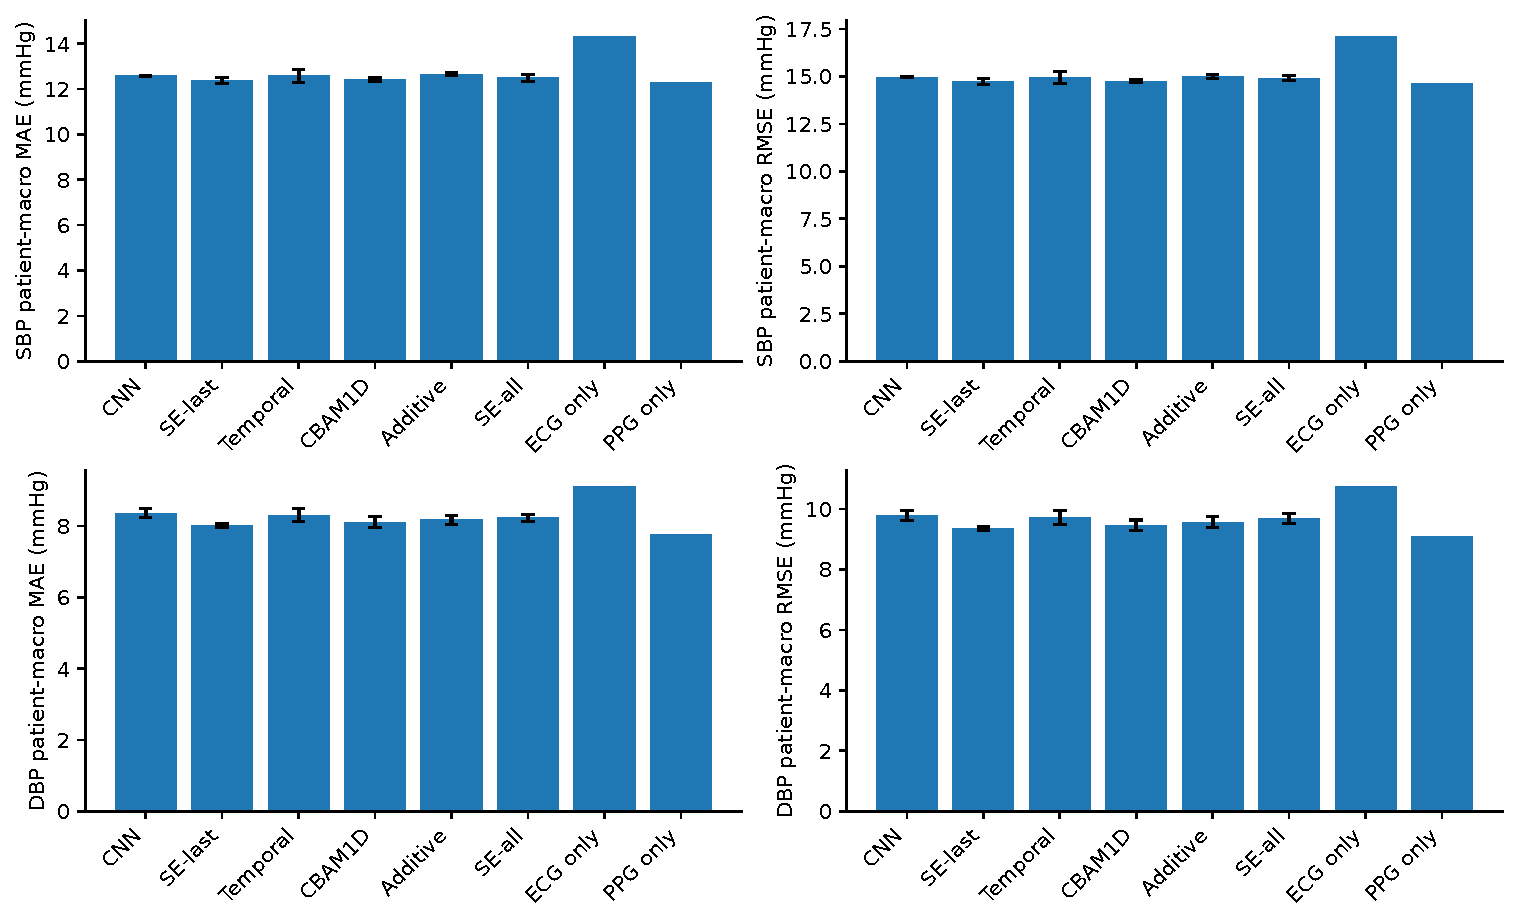
\includegraphics[width=\textwidth]{figures/attention_results.pdf}\caption{Primary-test patient-macro errors, averaged across seeds 42/43/44; error bars are sample seed SD. ECG-only/PPG-only results use seed 42 only and have no seed error bar. Test results do not determine selection.}\label{fig:attention_results}\end{figure*}

\begin{figure*}[t]\centering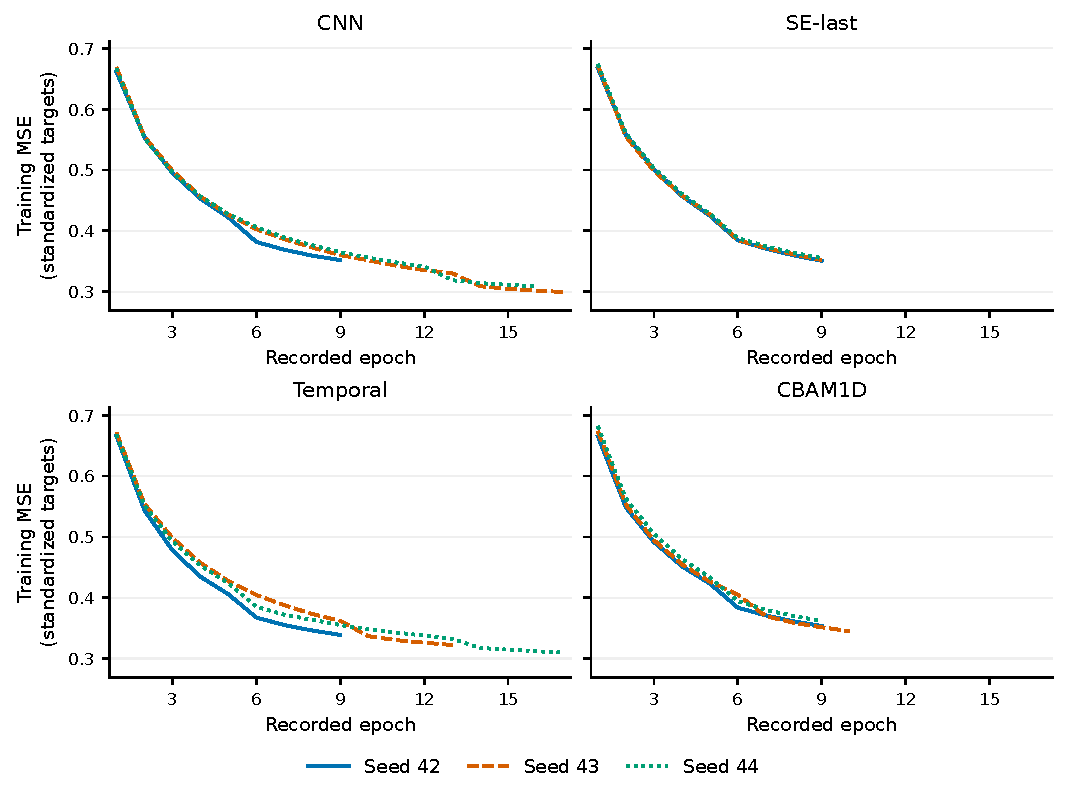
\includegraphics[width=\textwidth]{figures/attention_training_mse.pdf}\caption{Complete recorded training histories for the four primary architectures. Lines distinguish seeds and stop at their actual last epochs. MSE uses standardized targets and training-time augmentation; it is not measured in mmHg.}\label{fig:attention_training_mse}\end{figure*}

\begin{figure*}[t]\centering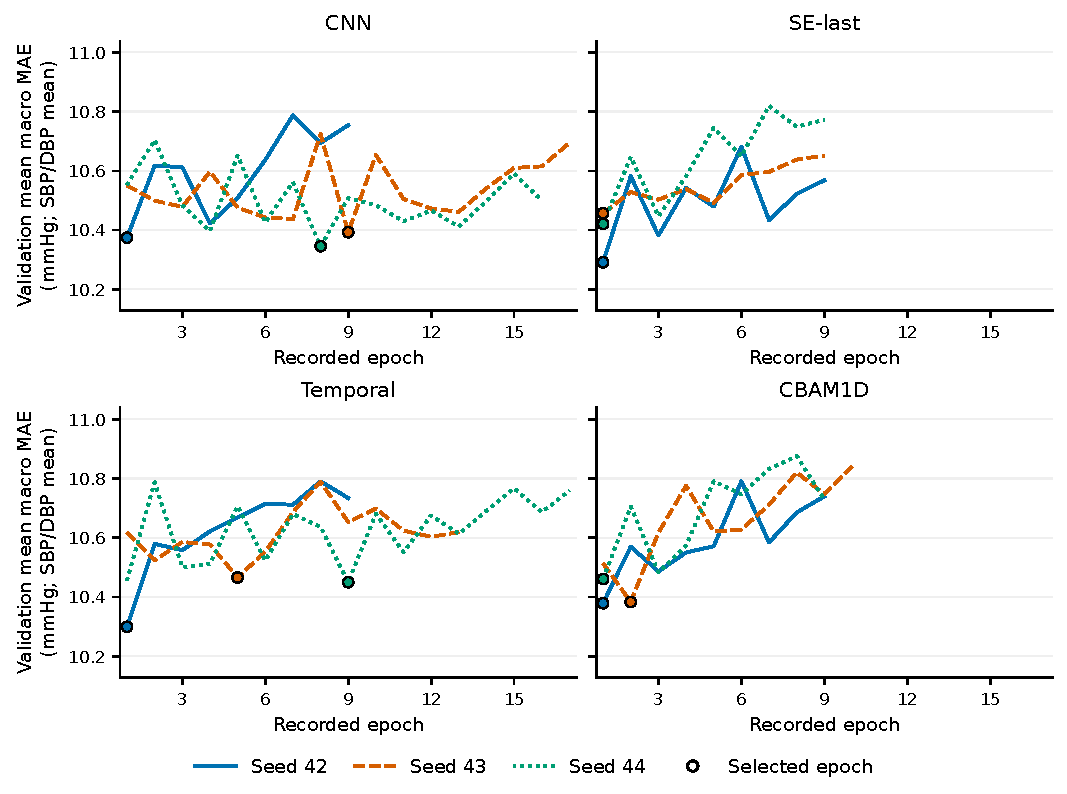
\includegraphics[width=\textwidth]{figures/attention_validation_mae.pdf}\caption{Complete validation histories for the same fixed fits. The ordinate averages patient-macro SBP and DBP MAE in mmHg. Circles mark saved validation-selected epochs; neither curves nor markers use test outcomes.}\label{fig:attention_validation_mae}\end{figure*}

\begin{figure*}[t]\centering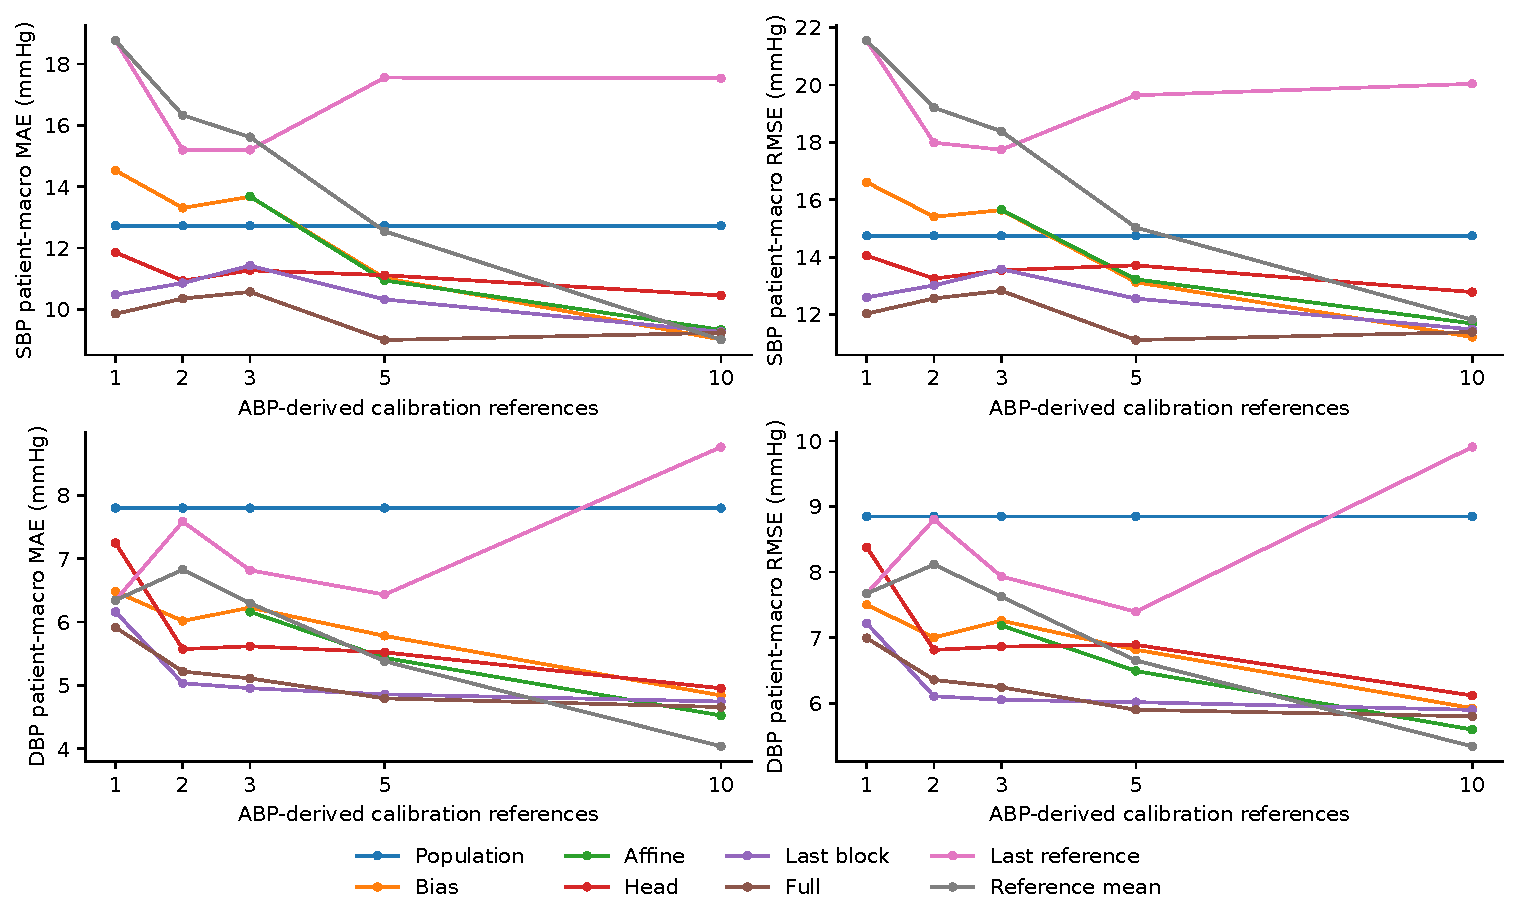
\includegraphics[width=\textwidth]{figures/personal_budget.pdf}\caption{Calibration-budget curves on common later queries. Every curve averages six patients equally and three seeds; reference age changes with nested budget.}\label{fig:personal_budget}\end{figure*}

\begin{figure*}[t]\centering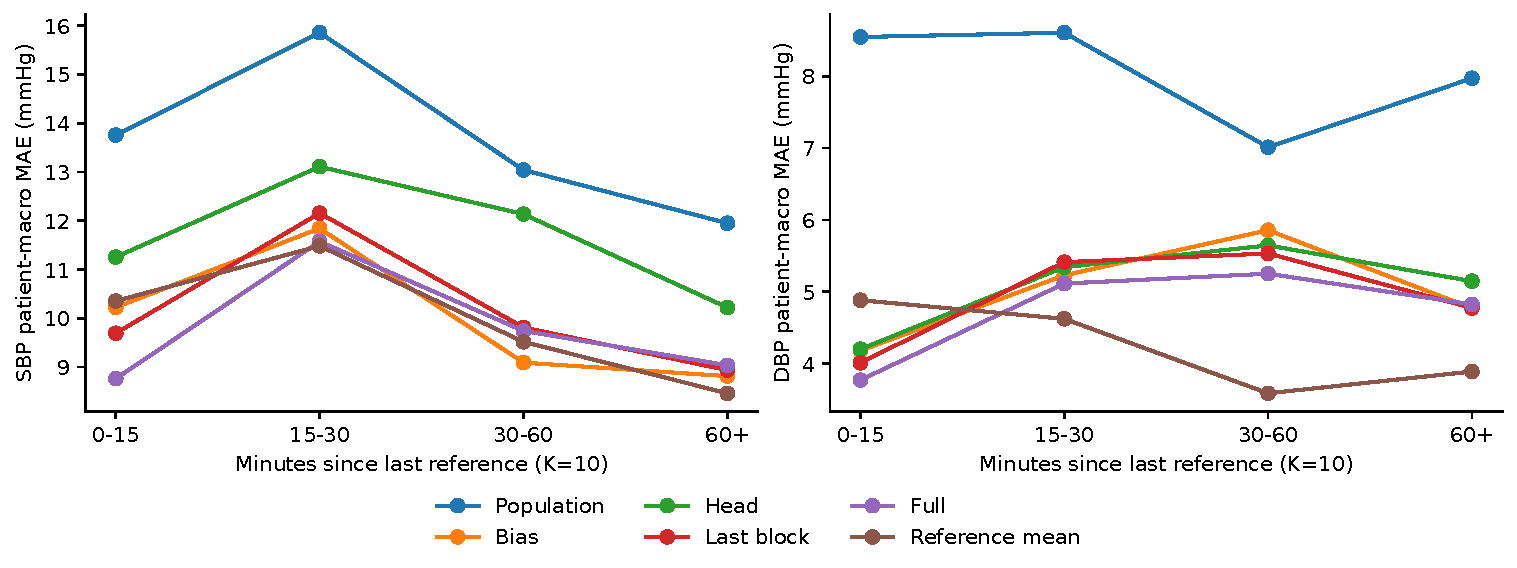
\includegraphics[width=\textwidth]{figures/personal_drift.pdf}\caption{Within-case error versus minutes since the actual final reference at K=10. Patient counts vary by interval; complete counts are saved with the results.}\label{fig:personal_drift}\end{figure*}

\begin{figure*}[t]\centering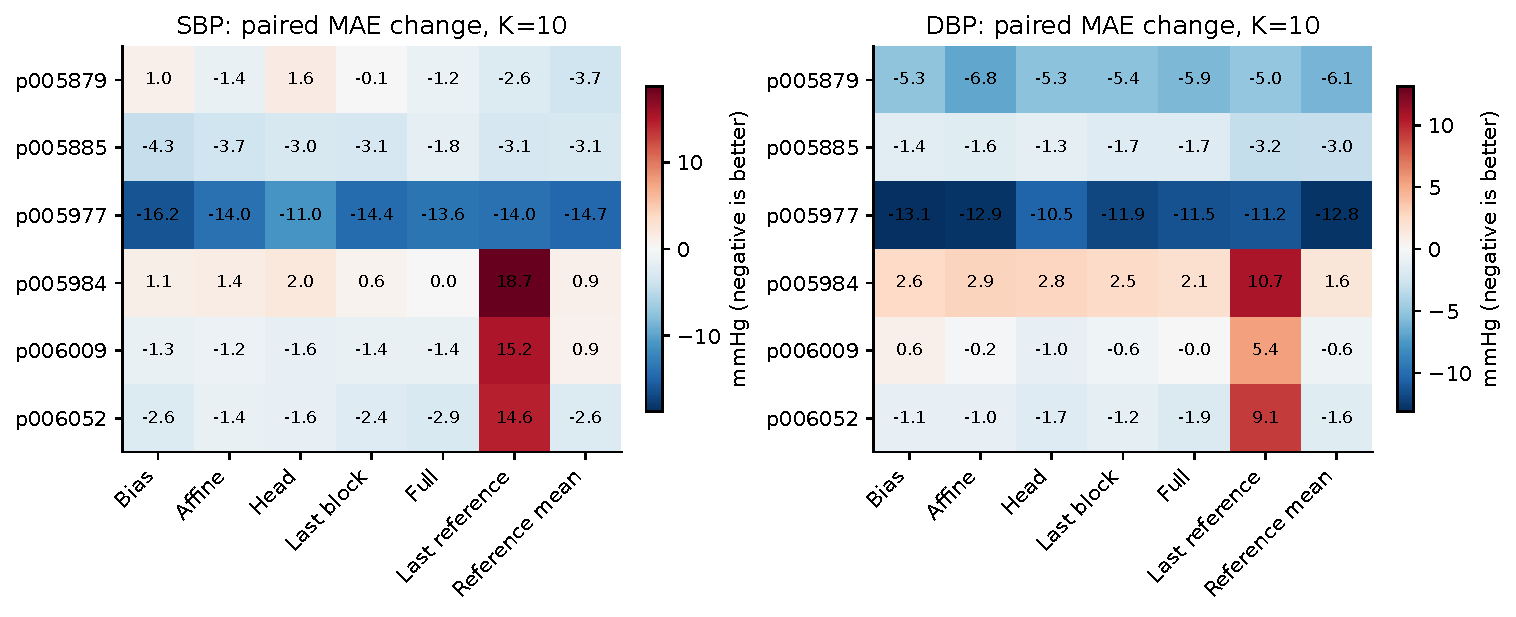
\includegraphics[width=\textwidth]{figures/patient_changes.pdf}\caption{Every final patient's paired change at K=10. Negative values improve on the matched population model; heterogeneous failures must not be hidden.}\label{fig:patient_changes}\end{figure*}

\begin{figure*}[t]\centering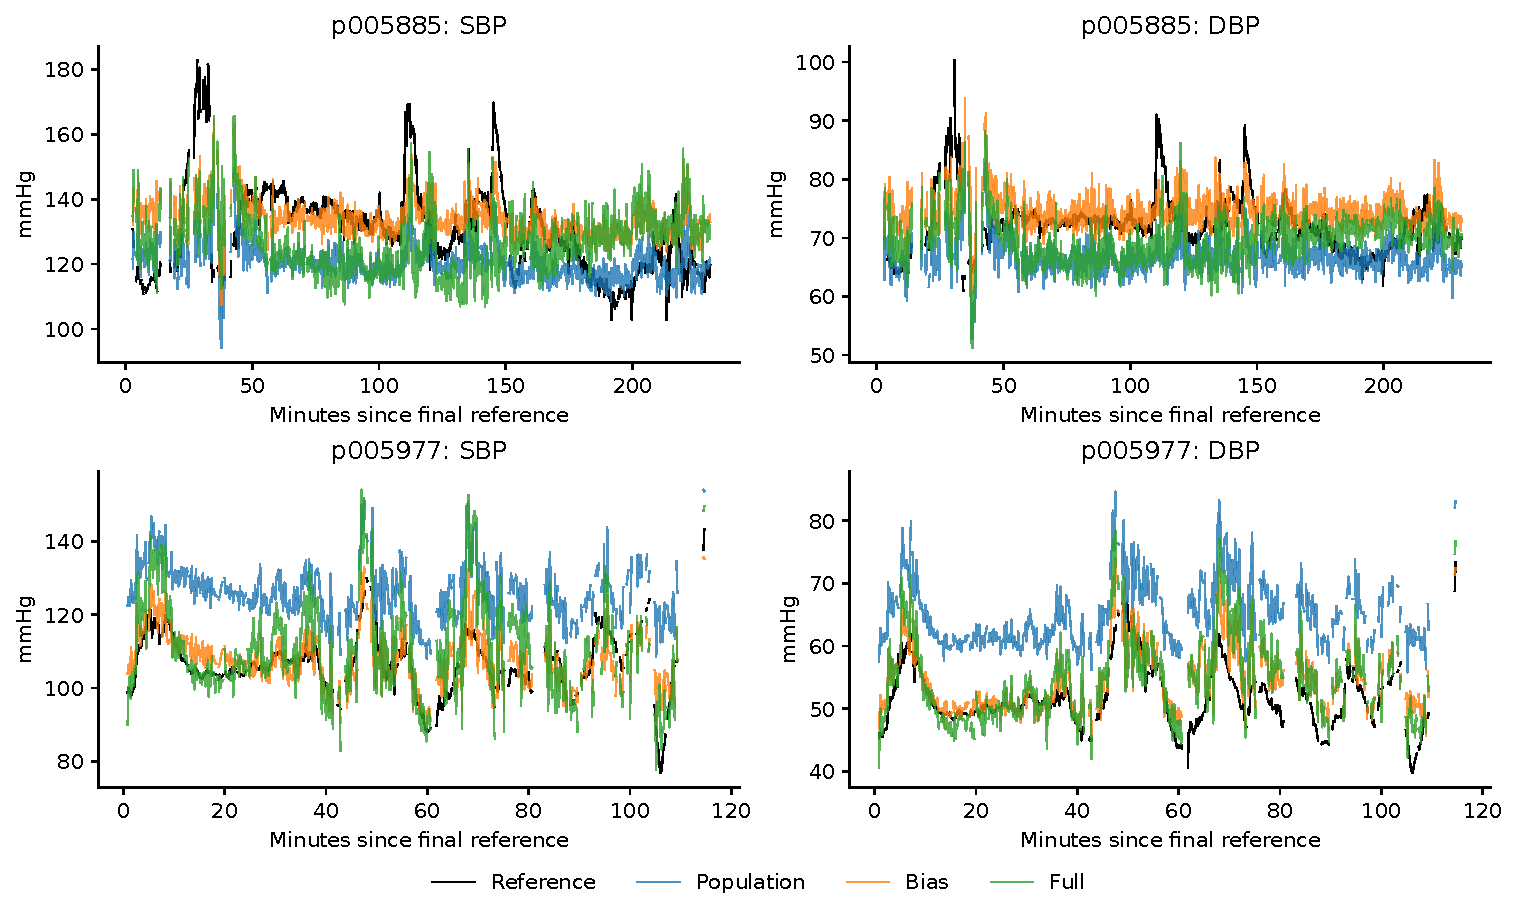
\includegraphics[width=\textwidth]{figures/temporal_examples.pdf}\caption{Representative upper-median and worst patients under baseline seed 42 query MAE, shown at K=10. Lines break at recording gaps. Bias and full-model alternatives were prespecified; no post-hoc time alignment is applied.}\label{fig:temporal_examples}\end{figure*}

\begin{figure*}[t]\centering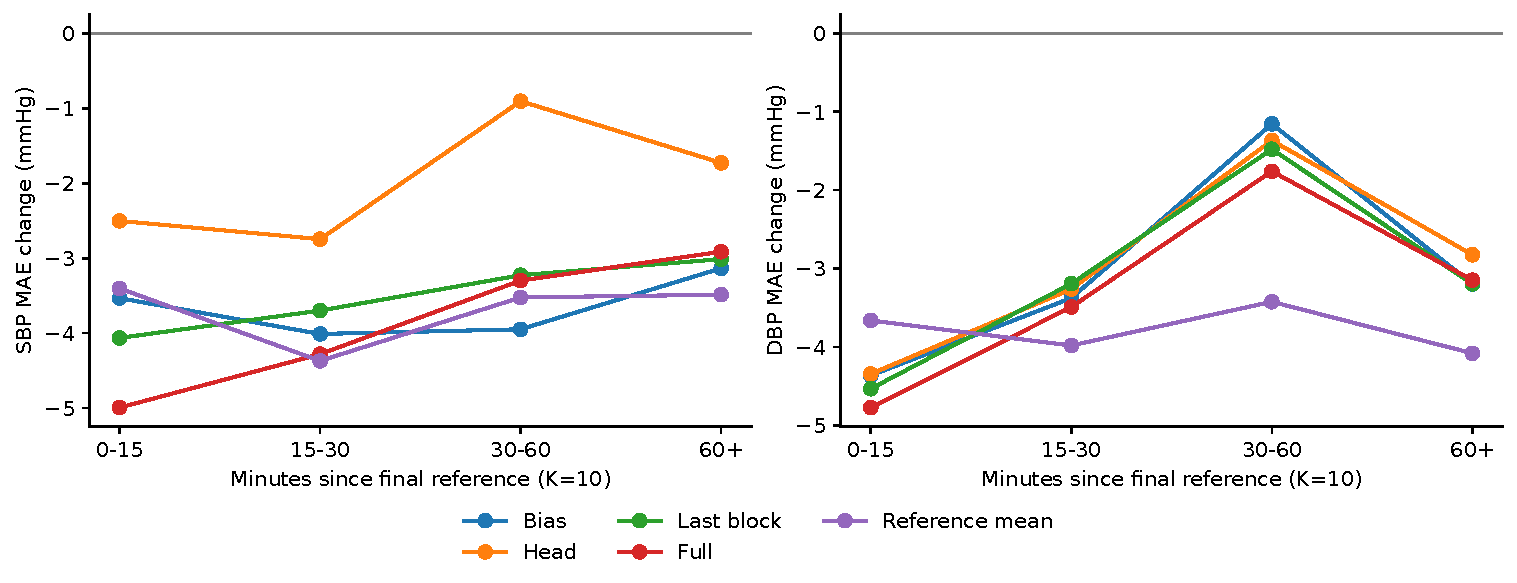
\includegraphics[width=\textwidth]{figures/drift_gain.pdf}\caption{Paired patient-macro MAE change versus the population model in each time interval, at K=10. Negative values favor calibration. Changing patient coverage is shown in the appendix.}\label{fig:drift_gain}\end{figure*}

\begin{figure*}[t]\centering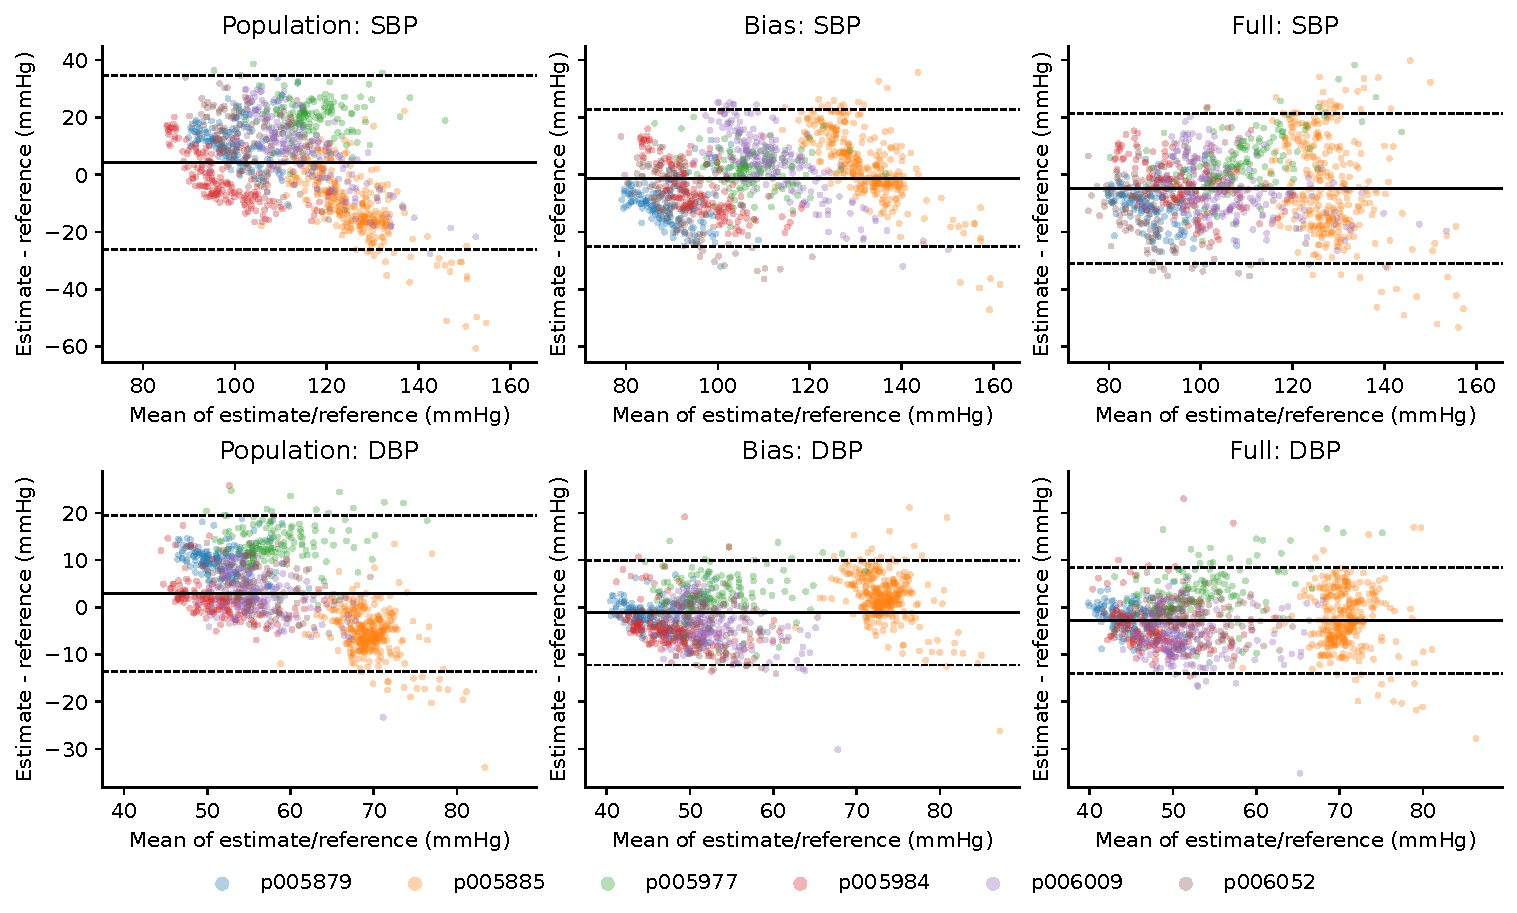
\includegraphics[width=\textwidth]{figures/repeated_bland_altman.pdf}\caption{Descriptive repeated-measurement Bland--Altman plots for seed 42, K=10. Colors identify the six patients. Every fourth window is displayed; all windows determine the bias and random-intercept limits of agreement. Serial dependence remains, so these are not confidence bounds or clinical validation limits.}\label{fig:repeated_bland_altman}\end{figure*}

\begin{figure*}[t]\centering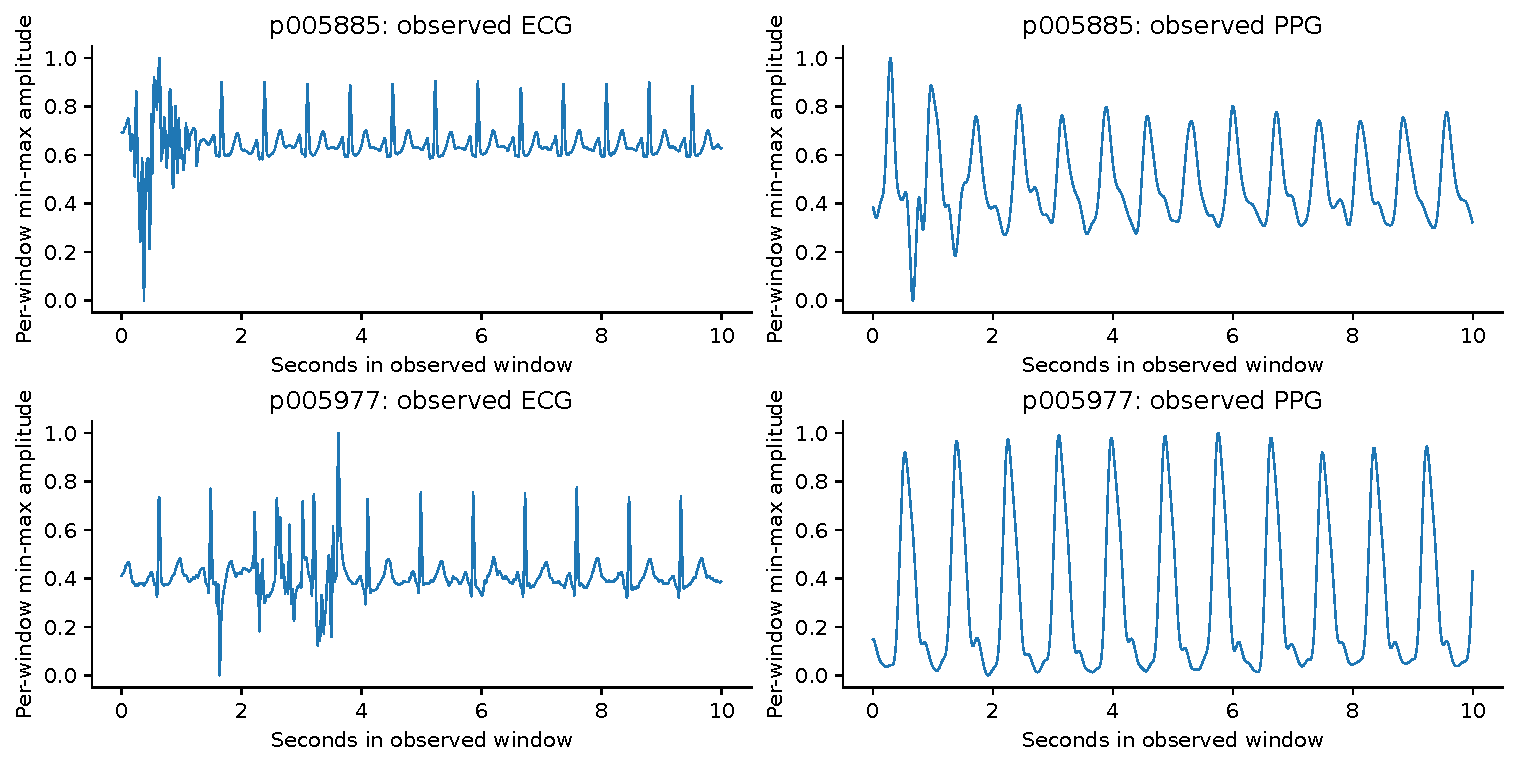
\includegraphics[width=\textwidth]{figures/observed_waveforms.pdf}\caption{Actual normalized ten-second ECG/PPG input windows from the prespecified example patients. These are observed signals, not predicted future waveforms. Corresponding scalar reference and prediction values are tabulated in the appendix.}\label{fig:observed_waveforms}\end{figure*}
\begin{table*}[t]\centering\scriptsize\setlength{\tabcolsep}{3pt}
\begin{tabular}{lrrrrrrrrrrrr}\toprule
SBP, test & MAE & RMSE & Bias & SD & MedAE & Q90 & Q95 & $\leq5$ & $\leq10$ & $\leq15$ & $r$ & $R^2$\\\midrule
CNN & 12.59 & 16.08 & -1.81 & 15.96 & 10.45 & 25.88 & 31.20 & 25.60 & 48.11 & 66.60 & 0.56 & 0.26\\
SE-last & 12.39 & 15.89 & -1.76 & 15.78 & 10.19 & 25.65 & 31.13 & 26.03 & 49.22 & 67.60 & 0.55 & 0.28\\
Temporal & 12.58 & 16.10 & -1.83 & 15.99 & 10.39 & 25.89 & 31.44 & 25.57 & 48.40 & 66.68 & 0.56 & 0.26\\
CBAM1D & 12.42 & 15.85 & -0.29 & 15.84 & 10.27 & 25.53 & 31.11 & 25.64 & 48.88 & 67.30 & 0.55 & 0.29\\
Additive & 12.66 & 16.17 & -1.03 & 16.12 & 10.43 & 26.42 & 32.06 & 25.47 & 48.24 & 66.68 & 0.55 & 0.26\\
SE-all & 12.49 & 16.01 & -1.64 & 15.92 & 10.27 & 25.89 & 31.40 & 25.87 & 48.88 & 67.10 & 0.56 & 0.27\\
ECG only & 14.31 & 18.21 & -0.02 & 18.21 & 11.87 & 29.28 & 35.60 & 22.22 & 42.97 & 60.60 & 0.32 & 0.06\\
PPG only & 12.30 & 15.69 & -1.13 & 15.65 & 10.23 & 25.07 & 30.68 & 25.38 & 48.97 & 67.94 & 0.55 & 0.30\\
\bottomrule\end{tabular}
\caption{Pooled-window SBP metrics on test, averaged across matched seeds (single seed for modality ablations). SD is sample error SD. Threshold columns are percentages. Complete per-patient and macro metrics are in the machine-readable results.}\end{table*}

\begin{table*}[t]\centering\scriptsize\setlength{\tabcolsep}{3pt}
\begin{tabular}{lrrrrrrrrrrrr}\toprule
DBP, test & MAE & RMSE & Bias & SD & MedAE & Q90 & Q95 & $\leq5$ & $\leq10$ & $\leq15$ & $r$ & $R^2$\\\midrule
CNN & 8.36 & 10.68 & -1.29 & 10.56 & 6.91 & 17.45 & 21.18 & 37.59 & 66.88 & 84.90 & 0.50 & 0.19\\
SE-last & 8.00 & 10.19 & -0.89 & 10.15 & 6.65 & 16.56 & 20.06 & 38.83 & 68.91 & 86.68 & 0.53 & 0.26\\
Temporal & 8.31 & 10.57 & -1.22 & 10.46 & 6.91 & 17.16 & 20.97 & 37.46 & 67.11 & 85.38 & 0.51 & 0.21\\
CBAM1D & 8.11 & 10.30 & -0.52 & 10.28 & 6.75 & 16.76 & 20.29 & 38.21 & 68.20 & 86.13 & 0.52 & 0.25\\
Additive & 8.18 & 10.47 & -1.00 & 10.42 & 6.72 & 17.05 & 20.80 & 38.63 & 67.95 & 85.59 & 0.51 & 0.22\\
SE-all & 8.23 & 10.52 & -1.13 & 10.46 & 6.79 & 17.26 & 20.99 & 38.34 & 67.61 & 85.32 & 0.51 & 0.21\\
ECG only & 9.10 & 11.54 & -0.01 & 11.54 & 7.53 & 18.95 & 22.98 & 34.39 & 62.76 & 81.27 & 0.31 & 0.05\\
PPG only & 7.77 & 9.76 & -1.36 & 9.66 & 6.64 & 15.65 & 19.00 & 38.36 & 69.81 & 88.44 & 0.58 & 0.32\\
\bottomrule\end{tabular}
\caption{Pooled-window DBP metrics on test, averaged across matched seeds (single seed for modality ablations). SD is sample error SD. Threshold columns are percentages. Complete per-patient and macro metrics are in the machine-readable results.}\end{table*}

\begin{table*}[t]\centering\scriptsize\setlength{\tabcolsep}{3pt}
\begin{tabular}{lrrrrrrrrrrrr}\toprule
SBP, aami & MAE & RMSE & Bias & SD & MedAE & Q90 & Q95 & $\leq5$ & $\leq10$ & $\leq15$ & $r$ & $R^2$\\\midrule
CNN & 18.34 & 24.70 & -11.27 & 21.97 & 13.59 & 40.32 & 53.79 & 19.12 & 37.54 & 54.65 & 0.71 & 0.36\\
SE-last & 19.46 & 26.33 & -13.22 & 22.76 & 14.43 & 43.08 & 55.30 & 17.82 & 35.79 & 51.75 & 0.69 & 0.27\\
Temporal & 18.55 & 24.73 & -11.46 & 21.92 & 14.29 & 39.38 & 53.13 & 18.12 & 36.09 & 51.60 & 0.71 & 0.36\\
CBAM1D & 18.75 & 25.14 & -11.16 & 22.51 & 14.20 & 40.54 & 53.55 & 18.12 & 35.54 & 52.25 & 0.70 & 0.33\\
Additive & 18.56 & 25.24 & -11.64 & 22.40 & 13.82 & 40.37 & 53.83 & 20.02 & 37.69 & 53.65 & 0.69 & 0.33\\
SE-all & 18.57 & 24.80 & -11.28 & 22.11 & 14.31 & 39.07 & 52.20 & 19.47 & 36.84 & 52.10 & 0.70 & 0.35\\
ECG only & 25.25 & 32.19 & -15.04 & 28.49 & 20.12 & 57.01 & 67.64 & 9.61 & 24.62 & 36.79 & 0.39 & -0.09\\
PPG only & 19.58 & 26.79 & -12.91 & 23.49 & 14.24 & 44.09 & 57.70 & 20.72 & 37.09 & 52.70 & 0.66 & 0.25\\
\bottomrule\end{tabular}
\caption{Pooled-window SBP metrics on aami, averaged across matched seeds (single seed for modality ablations). SD is sample error SD. Threshold columns are percentages. Complete per-patient and macro metrics are in the machine-readable results.}\end{table*}

\begin{table*}[t]\centering\scriptsize\setlength{\tabcolsep}{3pt}
\begin{tabular}{lrrrrrrrrrrrr}\toprule
DBP, aami & MAE & RMSE & Bias & SD & MedAE & Q90 & Q95 & $\leq5$ & $\leq10$ & $\leq15$ & $r$ & $R^2$\\\midrule
CNN & 12.15 & 15.46 & -7.64 & 13.42 & 10.10 & 24.26 & 30.29 & 24.42 & 49.60 & 70.02 & 0.68 & 0.28\\
SE-last & 12.42 & 16.14 & -8.21 & 13.90 & 10.03 & 25.75 & 32.31 & 25.23 & 49.65 & 69.92 & 0.66 & 0.21\\
Temporal & 12.32 & 15.72 & -7.64 & 13.71 & 10.30 & 25.29 & 31.05 & 24.22 & 48.80 & 69.52 & 0.66 & 0.25\\
CBAM1D & 12.06 & 15.61 & -7.45 & 13.72 & 10.11 & 24.45 & 31.36 & 25.33 & 49.15 & 70.57 & 0.67 & 0.26\\
Additive & 12.25 & 15.92 & -8.06 & 13.74 & 10.05 & 25.68 & 32.72 & 25.48 & 49.55 & 71.02 & 0.66 & 0.24\\
SE-all & 12.32 & 15.76 & -7.53 & 13.85 & 10.52 & 24.91 & 31.35 & 24.02 & 47.95 & 69.72 & 0.65 & 0.25\\
ECG only & 15.48 & 20.03 & -10.25 & 17.22 & 12.25 & 33.77 & 37.84 & 23.27 & 43.54 & 58.71 & 0.33 & -0.21\\
PPG only & 12.85 & 16.33 & -8.79 & 13.77 & 10.93 & 25.66 & 31.65 & 23.27 & 45.35 & 68.32 & 0.67 & 0.20\\
\bottomrule\end{tabular}
\caption{Pooled-window DBP metrics on aami, averaged across matched seeds (single seed for modality ablations). SD is sample error SD. Threshold columns are percentages. Complete per-patient and macro metrics are in the machine-readable results.}\end{table*}

\begin{table*}[t]\centering\small
\begin{tabular}{lrrrrrr}\toprule
SBP, K=10 & Macro MAE & Macro RMSE & Bias & Error SD & $\Delta$ MAE (95\% CI) & $\leq 10$\\\midrule
Population & 12.73 & 14.74 & 3.01 & 15.10 & Reference & 43.71\\
Bias & 9.02 & 11.22 & -1.63 & 11.57 & -3.71 [-9.04, 0.03] & 62.43\\
Affine & 9.34 & 11.69 & -1.76 & 12.02 & -3.39 [-8.02, -0.34] & 61.33\\
Head & 10.46 & 12.78 & -1.20 & 13.17 & -2.27 [-6.02, 0.67] & 54.96\\
Last block & 9.27 & 11.48 & -2.39 & 11.71 & -3.46 [-8.00, -0.45] & 61.75\\
Full & 9.24 & 11.39 & -3.14 & 11.65 & -3.49 [-7.65, -0.87] & 60.53\\
Last reference & 17.54 & 20.04 & 3.59 & 20.86 & 4.81 [-4.90, 14.40] & 41.34\\
Reference mean & 9.01 & 11.82 & -0.06 & 12.52 & -3.71 [-8.34, -0.33] & 65.17\\
\bottomrule\end{tabular}
\caption{Personal SBP results at ten simulated references. MAE/RMSE are patient-macro; Bias, Error SD and the within-10 percentage are pooled-window statistics. Entries average matched seeds. Paired changes are model minus population, averaged within patient across seeds before a 2,000-resample patient bootstrap. Intervals are descriptive for six patients.}\end{table*}

\begin{table*}[t]\centering\small
\begin{tabular}{lrrrrrr}\toprule
DBP, K=10 & Macro MAE & Macro RMSE & Bias & Error SD & $\Delta$ MAE (95\% CI) & $\leq 10$\\\midrule
Population & 7.80 & 8.85 & 3.77 & 8.48 & Reference & 71.23\\
Bias & 4.84 & 5.92 & -1.40 & 6.00 & -2.96 [-7.52, 0.65] & 89.64\\
Affine & 4.52 & 5.60 & -1.02 & 5.77 & -3.27 [-7.87, 0.52] & 91.49\\
Head & 4.95 & 6.12 & -0.29 & 6.35 & -2.84 [-6.53, 0.13] & 89.22\\
Last block & 4.75 & 5.90 & -1.10 & 5.89 & -3.05 [-7.15, 0.24] & 90.30\\
Full & 4.66 & 5.80 & -1.07 & 5.77 & -3.14 [-7.03, 0.10] & 90.74\\
Last reference & 8.76 & 9.91 & 1.73 & 9.92 & 0.96 [-5.45, 7.36] & 66.81\\
Reference mean & 4.04 & 5.34 & -1.01 & 5.30 & -3.76 [-7.85, -0.34] & 92.76\\
\bottomrule\end{tabular}
\caption{Personal DBP results at ten simulated references. MAE/RMSE are patient-macro; Bias, Error SD and the within-10 percentage are pooled-window statistics. Entries average matched seeds. Paired changes are model minus population, averaged within patient across seeds before a 2,000-resample patient bootstrap. Intervals are descriptive for six patients.}\end{table*}

\begin{table*}[t]\centering\scriptsize\setlength{\tabcolsep}{3pt}
\begin{tabular}{lrrrrrrrrrrrr}\toprule
SBP, K=10 & MAE & RMSE & Bias & SD & MedAE & Q90 & Q95 & $\leq5$ & $\leq10$ & $\leq15$ & $r$ & $R^2$\\\midrule
Population & 12.66 & 15.42 & 3.01 & 15.10 & 11.45 & 24.22 & 28.15 & 22.46 & 43.71 & 64.01 & 0.57 & 0.29\\
Bias & 9.14 & 11.69 & -1.63 & 11.57 & 7.48 & 19.46 & 22.98 & 35.82 & 62.43 & 80.54 & 0.82 & 0.59\\
Affine & 9.40 & 12.15 & -1.76 & 12.02 & 7.71 & 19.33 & 23.81 & 33.87 & 61.33 & 80.66 & 0.82 & 0.56\\
Head & 10.46 & 13.23 & -1.20 & 13.17 & 9.06 & 20.24 & 24.73 & 28.13 & 54.96 & 76.46 & 0.79 & 0.47\\
Last block & 9.47 & 11.99 & -2.39 & 11.71 & 7.90 & 19.14 & 23.57 & 31.24 & 61.75 & 80.96 & 0.81 & 0.57\\
Full & 9.63 & 12.11 & -3.14 & 11.65 & 8.20 & 19.23 & 23.55 & 30.97 & 60.53 & 80.64 & 0.79 & 0.55\\
Last reference & 16.55 & 21.16 & 3.59 & 20.86 & 13.58 & 35.31 & 41.77 & 22.46 & 41.34 & 52.99 & 0.38 & -0.34\\
Reference mean & 9.32 & 12.52 & -0.06 & 12.52 & 6.96 & 20.69 & 25.65 & 37.79 & 65.17 & 79.18 & 0.75 & 0.53\\
\bottomrule\end{tabular}
\caption{Complete pooled-window personal SBP metrics at K=10, averaged across three seeds. Thresholds are percentages; undefined correlations are marked unavailable. Reference-only controls may correlate when pooling different patient means, despite being constant within each patient.}\end{table*}

\begin{table*}[t]\centering\scriptsize\setlength{\tabcolsep}{3pt}
\begin{tabular}{lrrrrrrrrrrrr}\toprule
DBP, K=10 & MAE & RMSE & Bias & SD & MedAE & Q90 & Q95 & $\leq5$ & $\leq10$ & $\leq15$ & $r$ & $R^2$\\\midrule
Population & 7.47 & 9.36 & 3.77 & 8.48 & 6.31 & 15.86 & 18.49 & 41.19 & 71.23 & 88.36 & 0.63 & 0.24\\
Bias & 4.92 & 6.20 & -1.40 & 6.00 & 4.16 & 10.05 & 11.79 & 58.08 & 89.64 & 98.54 & 0.90 & 0.67\\
Affine & 4.58 & 5.88 & -1.02 & 5.77 & 3.79 & 9.54 & 11.48 & 61.85 & 91.49 & 98.67 & 0.89 & 0.70\\
Head & 4.98 & 6.40 & -0.29 & 6.35 & 4.12 & 10.19 & 12.27 & 58.35 & 89.22 & 97.88 & 0.88 & 0.65\\
Last block & 4.75 & 6.09 & -1.10 & 5.89 & 3.88 & 9.80 & 11.74 & 61.13 & 90.30 & 98.39 & 0.88 & 0.68\\
Full & 4.71 & 6.03 & -1.07 & 5.77 & 3.94 & 9.75 & 11.76 & 61.37 & 90.74 & 98.20 & 0.87 & 0.69\\
Last reference & 7.81 & 10.07 & 1.73 & 9.92 & 6.02 & 17.53 & 19.80 & 43.53 & 66.81 & 83.52 & 0.61 & 0.13\\
Reference mean & 3.96 & 5.40 & -1.01 & 5.30 & 2.99 & 8.62 & 11.48 & 71.34 & 92.76 & 97.97 & 0.88 & 0.75\\
\bottomrule\end{tabular}
\caption{Complete pooled-window personal DBP metrics at K=10, averaged across three seeds. Thresholds are percentages; undefined correlations are marked unavailable. Reference-only controls may correlate when pooling different patient means, despite being constant within each patient.}\end{table*}
\section{Computational cost and engineering verification}
\begin{table*}[t]\centering\small
\begin{tabular}{lrrrr}\toprule
Variant & Parameters & Actual epochs & Selected epochs & Total training minutes\\\midrule
CNN & 37,666 & 9,17,16 & 1,9,8 & 49.1\\
SE-last & 38,296 & 9,9,9 & 1,1,1 & 26.4\\
Temporal & 37,680 & 9,13,17 & 1,5,9 & 54.6\\
CBAM1D & 38,310 & 9,10,9 & 1,2,1 & 31.0\\
Additive & 38,296 & 9,9,11 & 1,1,3 & 41.2\\
SE-all & 38,670 & 9,13,14 & 1,5,6 & 63.1\\
ECG only & 37,666 & 9 & 1 & 13.0\\
PPG only & 37,666 & 9 & 1 & 9.7\\
\bottomrule\end{tabular}
\caption{Real fitting costs across included seeds. Training time includes per-epoch validation and checkpointing. Complete CPU/accelerator inference timings and memory definitions are in the result JSON.}\end{table*}
The recorded environment is an Apple M5 with 24 GiB memory and PyTorch 2.14.0.
Population fitting uses MPS; personal adaptation uses CPU. Measured desktop
costs are not Raspberry Pi timings. Personal CPU execution overlapped later
MPS population fits, and other local jobs were active during part of the suite.
The saved timing ranges therefore include shared-host workload variation,
rather than isolated-hardware benchmarks.
Full source waveform hashes and patient
selection hashes are verified. Tests cover V1 equality, attention shapes and
counts, split separation, label/time alignment, support-only fitting, exact
hand-computed metrics, frozen BN and parameters, and epoch-resume equality.
No toy-test outputs enter the real inventory. The development and final
personal phases require 1,068 and 684 completed units respectively.
The personal inference CLI applies saved weights or correction coefficients
without later labels. All eight K=10/seed-42 strategies for the first frozen
target reproduced all 654 saved query predictions bitwise on CPU; source
artifacts remained unchanged. This replay is an engineering consistency
check, not another independent accuracy experiment.

\section{Interpretation and limitations}
Across the six required three-seed models, the lowest observed primary-test MAEs are SBP 12.386 mmHg for SE-last and DBP 8.002 mmHg for SE-last. These are descriptive endpoint-wise minima among prespecified fitted models, not a new model-selection rule or evidence of global superiority. Capacity and placement controls retain their distinct roles; supplementary ECA and single-seed sensor ablations do not enter this six-model summary. For SBP, SE-last minus CNN is -0.199 [-0.480, +0.068] mmHg. SE-last's observed SBP MAE is lower than CNN's (change -0.199 mmHg); its paired interval includes or touches zero. For DBP, SE-last minus CNN is -0.359 [-0.534, -0.184] mmHg. SE-last's observed DBP MAE is lower than CNN's (change -0.359 mmHg); its paired interval is wholly below zero. All intervals compare a fixed model with CNN, not the lowest model with every competitor; they are descriptive, conditional on the fitted seeds, and not adjusted for multiple comparisons or selecting an observed minimum. An interval including zero leaves the direction uncertain without erasing the observed point estimate. A validation-selected model need not have the lowest test error, and a lower observed test error is not a deployment-selection decision.

The controlled attention intervention tests mechanisms, placement, modality
availability and matched parameter count; equal capacity does not guarantee
equal optimization. Validation ranking is a prospective selection rule, not
a declaration that the selected architecture is globally best. The full
prespecified test comparison supplies separate evidence about generalization;
neither a favorable point estimate nor a validation ranking alone establishes
clinical usefulness or deployment readiness.
The per-patient table and calibration curves, not a single best number,
determine whether deeper adaptation consistently helps. A neural strategy
that fails to outperform reference-only controls adds complexity without
demonstrated incremental predictive value on this pilot. High-pressure and
low-pressure strata can reveal failures concealed by overall averages.

Six personal targets cannot establish a universal calibration budget or
durability time. The references are real invasive labels sampled to simulate
sparse calibration, whereas the intended Notre Dame student measurements will use cuffs. Sensor,
population and reference differences remain separate transfer questions.
Provided offline filtering, upstream reference-based quality selection and
an incompletely documented resampling kernel constrain online interpretation.
The study evaluates later known ECG/PPG, not future waveforms. It does not
test across visits or establish clinical certification. Exact negative,
inconsistent and positive effects are retained in saved per-patient outputs.

\section{Reproduction and artifact traceability}
The review/protocol gate is commit \texttt{1b93cf1}. The repository preserves V1 and uses
a dedicated research branch. Follow the README commands with Python 3.12 and
the pinned requirements. Run unit tests, the population stage, then personal
development and test; build this report only after the full real inventory
passes hash checks. Raw recordings, detailed predictions and model weights
remain outside Git under the documented artifact root. Committed JSON
summaries retain run/config/checkpoint hashes and per-patient metrics.
\onecolumn\appendix\section{Complete paired, pressure-range and budget results}\label{sec:complete}
\begin{table}[!htbp]\centering\small
\begin{tabular}{lrrrr}\toprule
Model & SBP MAE & DBP MAE & SBP RMSE & DBP RMSE\\\midrule
CNN & 12.59 $\pm$ 0.02 & 8.36 $\pm$ 0.12 & 14.96 $\pm$ 0.02 & 9.79 $\pm$ 0.17\\
SE-last & 12.39 $\pm$ 0.14 & 8.00 $\pm$ 0.05 & 14.72 $\pm$ 0.15 & 9.34 $\pm$ 0.06\\
Temporal & 12.58 $\pm$ 0.27 & 8.31 $\pm$ 0.19 & 14.96 $\pm$ 0.31 & 9.72 $\pm$ 0.24\\
CBAM1D & 12.42 $\pm$ 0.07 & 8.11 $\pm$ 0.15 & 14.74 $\pm$ 0.08 & 9.46 $\pm$ 0.17\\
Additive & 12.66 $\pm$ 0.06 & 8.18 $\pm$ 0.13 & 15.00 $\pm$ 0.09 & 9.57 $\pm$ 0.18\\
SE-all & 12.49 $\pm$ 0.14 & 8.23 $\pm$ 0.10 & 14.89 $\pm$ 0.14 & 9.68 $\pm$ 0.17\\
ECG only & 14.31 & 9.10 & 17.09 & 10.74\\
PPG only & 12.30 & 7.77 & 14.61 & 9.08\\
\bottomrule\end{tabular}
\caption{Primary-test patient-macro errors (mmHg), mean and sample SD across training seeds. The modality ablations have one seed. These SDs describe training variability, not patient uncertainty.}\end{table}

\begin{table}[!htbp]\centering\small
\begin{tabular}{lrr}\toprule
Model minus CNN & SBP change [95\% CI] & DBP change [95\% CI]\\\midrule
SE-last & -0.20 [-0.48, 0.07] & -0.36 [-0.53, -0.18]\\
Temporal & -0.01 [-0.19, 0.19] & -0.06 [-0.18, 0.07]\\
CBAM1D & -0.17 [-0.47, 0.13] & -0.25 [-0.43, -0.08]\\
Additive & 0.07 [-0.20, 0.32] & -0.18 [-0.34, -0.02]\\
SE-all & -0.09 [-0.28, 0.09] & -0.13 [-0.27, 0.00]\\
ECG only & 1.71 [0.84, 2.52] & 0.87 [0.19, 1.57]\\
PPG only & -0.31 [-0.79, 0.20] & -0.46 [-0.84, -0.07]\\
\bottomrule\end{tabular}
\caption{Patient-paired MAE changes (mmHg) on the primary test. Negative values favor the intervention. Three-seed comparisons average seeds 42/43/44 within patient; ECG-only/PPG-only ablations compare seed 42 only. The bootstrap resamples 141 patients, not windows.}\end{table}

\begin{table}[!htbp]\centering\small
\begin{tabular}{lrr}\toprule
Model minus CNN & SBP change [95\% CI] & DBP change [95\% CI]\\\midrule
SE-last & -0.24 [-0.53, 0.02] & -0.45 [-0.62, -0.27]\\
Temporal & 0.00 [-0.20, 0.20] & -0.07 [-0.19, 0.05]\\
CBAM1D & -0.21 [-0.52, 0.08] & -0.33 [-0.50, -0.15]\\
Additive & 0.04 [-0.23, 0.29] & -0.22 [-0.39, -0.07]\\
SE-all & -0.06 [-0.25, 0.12] & -0.11 [-0.24, 0.02]\\
ECG only & 2.14 [1.29, 2.98] & 1.15 [0.49, 1.82]\\
PPG only & -0.34 [-0.82, 0.18] & -0.51 [-0.86, -0.14]\\
\bottomrule\end{tabular}
\caption{Patient-paired RMSE changes (mmHg) on the primary test. Negative values favor the intervention. Three-seed comparisons average seeds 42/43/44 within patient; ECG-only/PPG-only ablations compare seed 42 only. The bootstrap resamples 141 patients, not windows.}\end{table}

\begin{table}[!htbp]\centering\small
\begin{tabular}{lrrrrr}\toprule
SBP stratum & Windows & Patients & MAE & RMSE & Bias\\\midrule
CNN: below 100 & 12172 & 128 & 13.40 & 16.63 & 11.63\\
CNN: 100 to below 140 & 38427 & 141 & 10.62 & 13.30 & -2.84\\
CNN: 140 or above & 5801 & 113 & 23.86 & 27.53 & -23.16\\
\bottomrule\end{tabular}
\caption{Primary-test SBP pressure-range errors (mmHg), averaged across seeds. Stratum errors are pooled within each label-defined range; counts are not multiplied by seeds. Only the unchanged baseline and validation-selected architecture are shown; all models are in the JSON.}\end{table}

\begin{table}[!htbp]\centering\small
\begin{tabular}{lrrrrr}\toprule
DBP stratum & Windows & Patients & MAE & RMSE & Bias\\\midrule
CNN: below 60 & 22970 & 135 & 7.70 & 9.90 & 6.00\\
CNN: 60 to below 90 & 32224 & 138 & 8.35 & 10.41 & -5.75\\
CNN: 90 or above & 1206 & 61 & 21.11 & 23.43 & -21.01\\
\bottomrule\end{tabular}
\caption{Primary-test DBP pressure-range errors (mmHg), averaged across seeds. Stratum errors are pooled within each label-defined range; counts are not multiplied by seeds. Only the unchanged baseline and validation-selected architecture are shown; all models are in the JSON.}\end{table}

\begin{table}[!htbp]\centering\scriptsize
\begin{tabular}{lrrrr}\toprule
SBP stratum, K=10 & Windows & Patients & MAE & RMSE\\\midrule
Population: below 100 & 1448 & 5 & 12.80 & 15.18\\
Population: 100 to below 140 & 2588 & 6 & 11.25 & 13.61\\
Population: 140 or above & 248 & 4 & 26.56 & 28.64\\
Bias: below 100 & 1448 & 5 & 7.90 & 9.65\\
Bias: 100 to below 140 & 2588 & 6 & 9.36 & 12.05\\
Bias: 140 or above & 248 & 4 & 13.98 & 17.02\\
Head: below 100 & 1448 & 5 & 9.62 & 11.41\\
Head: 100 to below 140 & 2588 & 6 & 10.51 & 13.65\\
Head: 140 or above & 248 & 4 & 14.80 & 17.46\\
Last block: below 100 & 1448 & 5 & 7.72 & 9.40\\
Last block: 100 to below 140 & 2588 & 6 & 9.76 & 12.35\\
Last block: 140 or above & 248 & 4 & 16.71 & 19.17\\
Full: below 100 & 1448 & 5 & 6.79 & 8.43\\
Full: 100 to below 140 & 2588 & 6 & 10.17 & 12.32\\
Full: 140 or above & 248 & 4 & 20.55 & 23.04\\
Reference mean: below 100 & 1448 & 5 & 6.63 & 8.57\\
Reference mean: 100 to below 140 & 2588 & 6 & 9.85 & 12.69\\
Reference mean: 140 or above & 248 & 4 & 19.46 & 24.45\\
\bottomrule\end{tabular}
\caption{Personal-query SBP pressure-range errors (mmHg), averaged across seeds. Empty reference-pressure ranges are unavailable, not perfect performance. More than one range may contain the same patient.}\end{table}

\begin{table}[!htbp]\centering\scriptsize
\begin{tabular}{lrrrr}\toprule
DBP stratum, K=10 & Windows & Patients & MAE & RMSE\\\midrule
Population: below 60 & 2801 & 5 & 8.21 & 10.18\\
Population: 60 to below 90 & 1477 & 6 & 6.01 & 7.41\\
Population: 90 or above & 6 & 1 & 21.81 & 22.50\\
Bias: below 60 & 2801 & 5 & 4.63 & 5.66\\
Bias: 60 to below 90 & 1477 & 6 & 5.45 & 7.04\\
Bias: 90 or above & 6 & 1 & 13.60 & 14.69\\
Head: below 60 & 2801 & 5 & 4.85 & 6.06\\
Head: 60 to below 90 & 1477 & 6 & 5.20 & 6.92\\
Head: 90 or above & 6 & 1 & 12.92 & 13.96\\
Last block: below 60 & 2801 & 5 & 4.62 & 5.73\\
Last block: 60 to below 90 & 1477 & 6 & 4.95 & 6.61\\
Last block: 90 or above & 6 & 1 & 15.39 & 16.28\\
Full: below 60 & 2801 & 5 & 4.57 & 5.71\\
Full: 60 to below 90 & 1477 & 6 & 4.91 & 6.48\\
Full: 90 or above & 6 & 1 & 17.64 & 18.47\\
Reference mean: below 60 & 2801 & 5 & 3.45 & 4.29\\
Reference mean: 60 to below 90 & 1477 & 6 & 4.87 & 6.94\\
Reference mean: 90 or above & 6 & 1 & 19.11 & 19.45\\
\bottomrule\end{tabular}
\caption{Personal-query DBP pressure-range errors (mmHg), averaged across seeds. Empty reference-pressure ranges are unavailable, not perfect performance. More than one range may contain the same patient.}\end{table}

\begin{table}[!htbp]\centering\scriptsize
\begin{tabular}{lrrrrrrrr}\toprule
Age from last reference & Windows & Patients & Pop. S & Pop. D & Bias S & Bias D & Full S & Full D\\\midrule
K=1, 0--15 min & 0 & 0 & -- & -- & -- & -- & -- & --\\
K=1, 15--30 min & 62 & 3 & 18.90 & 12.76 & 13.67 & 7.70 & 9.29 & 8.97\\
K=1, 30--60 min & 626 & 6 & 12.42 & 7.05 & 13.05 & 7.30 & 8.99 & 5.34\\
K=1, 60+ min & 3596 & 6 & 12.16 & 7.66 & 14.69 & 6.53 & 9.71 & 5.96\\
K=5, 0--15 min & 33 & 1 & 10.21 & 4.94 & 22.17 & 6.62 & 15.65 & 6.93\\
K=5, 15--30 min & 280 & 4 & 16.17 & 10.15 & 9.53 & 4.21 & 7.86 & 3.87\\
K=5, 30--60 min & 739 & 6 & 11.75 & 6.84 & 11.93 & 6.77 & 8.22 & 4.43\\
K=5, 60+ min & 3232 & 6 & 12.21 & 7.77 & 11.22 & 5.81 & 8.75 & 4.76\\
K=10, 0--15 min & 352 & 5 & 13.76 & 8.55 & 10.23 & 4.18 & 8.77 & 3.77\\
K=10, 15--30 min & 379 & 5 & 15.86 & 8.61 & 11.85 & 5.23 & 11.58 & 5.11\\
K=10, 30--60 min & 781 & 6 & 13.04 & 7.01 & 9.09 & 5.86 & 9.74 & 5.25\\
K=10, 60+ min & 2772 & 6 & 11.95 & 7.97 & 8.82 & 4.77 & 9.04 & 4.82\\
\bottomrule\end{tabular}
\caption{Drift-bin coverage and patient-macro MAE (mmHg) at three budgets. S/D mean SBP/DBP. Counts are unique windows/patients, not multiplied by seeds. Differences across intervals also reflect which patients remain observed.}\end{table}

\begin{table}[!htbp]\centering\scriptsize
\begin{tabular}{lrrrrrr}\toprule
Patient (role) & Case & Windows & Observed min & Elapsed min & Queries & Early span min\\\midrule
p005548 (Dev) & c4678 & 584 & 97.33 & 136.33 & 481 & 27.27\\
p005647 (Dev) & c4746 & 703 & 117.17 & 240.33 & 486 & 48.07\\
p005968 (Dev) & c3618 & 498 & 83.00 & 109.50 & 401 & 21.90\\
p006090 (Dev) & c2134 & 624 & 104.00 & 161.00 & 487 & 32.20\\
p005879 (Test) & c5552 & 806 & 134.33 & 145.00 & 654 & 29.00\\
p005885 (Test) & c0637 & 1449 & 241.50 & 288.00 & 1220 & 57.60\\
p005977 (Test) & c3725 & 721 & 120.17 & 144.17 & 569 & 28.83\\
p005984 (Test) & c4777 & 797 & 132.83 & 179.83 & 666 & 35.97\\
p006009 (Test) & c2935 & 820 & 136.67 & 265.50 & 761 & 53.10\\
p006052 (Test) & c4462 & 510 & 85.00 & 100.33 & 414 & 20.07\\
\bottomrule\end{tabular}
\caption{Chronological personal cohort. Observed duration counts retained ten-second windows; elapsed duration includes gaps. Every patient has ten available spaced reference windows; K selects a nested prefix. Queries are identical across all methods and budgets, and all ten patients were excluded from population fitting.}\end{table}

\begin{table}[!htbp]\centering\small
\begin{tabular}{lrrrrr}\toprule
Patient & Source row & Reference S/D & Population & Bias & Full\\\midrule
p005885 & 229 & 133.91/71.62 & 130.33/70.96 & 143.74/78.67 & 166.14/76.28\\
p005977 & 152 & 98.80/45.32 & 122.43/57.43 & 103.93/46.75 & 90.01/40.64\\
\bottomrule\end{tabular}
\caption{Scalar SBP/DBP values (mmHg) paired with the observed-waveform figure. These are the first later query windows of the upper-median and worst patients under seed-42 population MAE, not windows selected for a favorable prediction.}\end{table}
Nested budgets change both reference count and last-reference age: these curves are not a pure sample-complexity experiment. Primary reference-relative bins and secondary boundary-relative bins expose this distinction; no clinical minimum cuff count is inferred.

\begin{table}[!htbp]\centering\small
\begin{tabular}{lrrrrr}\toprule
SBP MAE & K=1 & K=2 & K=3 & K=5 & K=10\\\midrule
Population & $12.73\pm0.74$ & $12.73\pm0.74$ & $12.73\pm0.74$ & $12.73\pm0.74$ & $12.73\pm0.74$\\
Bias & $14.53\pm0.67$ & $13.31\pm0.81$ & $13.68\pm1.16$ & $11.02\pm0.82$ & $9.02\pm0.51$\\
Affine & -- & -- & $13.69\pm1.14$ & $10.95\pm0.66$ & $9.34\pm0.39$\\
Head & $11.86\pm0.29$ & $10.94\pm1.34$ & $11.28\pm0.99$ & $11.12\pm1.26$ & $10.46\pm0.95$\\
Last block & $10.48\pm1.62$ & $10.86\pm2.53$ & $11.43\pm2.30$ & $10.33\pm1.65$ & $9.27\pm0.79$\\
Full & $9.86\pm1.29$ & $10.36\pm2.62$ & $10.57\pm2.29$ & $9.01\pm0.95$ & $9.24\pm1.50$\\
Last reference & $18.76\pm0.00$ & $15.20\pm0.00$ & $15.20\pm0.00$ & $17.56\pm0.00$ & $17.54\pm0.00$\\
Reference mean & $18.76\pm0.00$ & $16.33\pm0.00$ & $15.62\pm0.00$ & $12.55\pm0.00$ & $9.01\pm0.00$\\
\bottomrule\end{tabular}
\caption{All-budget patient-macro SBP MAE in mmHg: mean $\pm$ sample SD across three matched population seeds, after equal weighting of the six final patients within each seed. Seed SD is not a patient confidence interval. Affine calibration is prespecified as unavailable for K below three.}\end{table}

\begin{table}[!htbp]\centering\small
\begin{tabular}{lrrrrr}\toprule
SBP RMSE & K=1 & K=2 & K=3 & K=5 & K=10\\\midrule
Population & $14.74\pm0.67$ & $14.74\pm0.67$ & $14.74\pm0.67$ & $14.74\pm0.67$ & $14.74\pm0.67$\\
Bias & $16.61\pm0.71$ & $15.41\pm0.77$ & $15.64\pm1.14$ & $13.13\pm0.73$ & $11.22\pm0.46$\\
Affine & -- & -- & $15.66\pm1.13$ & $13.23\pm0.44$ & $11.69\pm0.36$\\
Head & $14.05\pm0.27$ & $13.25\pm1.50$ & $13.54\pm1.22$ & $13.72\pm1.85$ & $12.78\pm1.16$\\
Last block & $12.60\pm1.72$ & $13.02\pm2.52$ & $13.58\pm2.36$ & $12.56\pm1.93$ & $11.48\pm1.09$\\
Full & $12.03\pm1.48$ & $12.56\pm2.74$ & $12.83\pm2.48$ & $11.11\pm1.09$ & $11.39\pm1.65$\\
Last reference & $21.54\pm0.00$ & $17.99\pm0.00$ & $17.74\pm0.00$ & $19.64\pm0.00$ & $20.04\pm0.00$\\
Reference mean & $21.54\pm0.00$ & $19.21\pm0.00$ & $18.39\pm0.00$ & $15.03\pm0.00$ & $11.82\pm0.00$\\
\bottomrule\end{tabular}
\caption{All-budget patient-macro SBP RMSE in mmHg: mean $\pm$ sample SD across three matched population seeds, after equal weighting of the six final patients within each seed. Seed SD is not a patient confidence interval. Affine calibration is prespecified as unavailable for K below three.}\end{table}

\begin{table}[!htbp]\centering\small
\begin{tabular}{lrrrrr}\toprule
DBP MAE & K=1 & K=2 & K=3 & K=5 & K=10\\\midrule
Population & $7.80\pm1.11$ & $7.80\pm1.11$ & $7.80\pm1.11$ & $7.80\pm1.11$ & $7.80\pm1.11$\\
Bias & $6.48\pm0.60$ & $6.02\pm0.73$ & $6.23\pm0.66$ & $5.78\pm0.82$ & $4.84\pm0.47$\\
Affine & -- & -- & $6.16\pm0.58$ & $5.43\pm0.39$ & $4.52\pm0.11$\\
Head & $7.25\pm0.31$ & $5.57\pm0.65$ & $5.62\pm0.58$ & $5.52\pm0.51$ & $4.95\pm0.18$\\
Last block & $6.16\pm1.04$ & $5.03\pm0.47$ & $4.95\pm0.46$ & $4.86\pm0.70$ & $4.75\pm0.46$\\
Full & $5.91\pm1.25$ & $5.22\pm0.43$ & $5.11\pm0.11$ & $4.80\pm0.35$ & $4.66\pm0.41$\\
Last reference & $6.34\pm0.00$ & $7.58\pm0.00$ & $6.82\pm0.00$ & $6.43\pm0.00$ & $8.76\pm0.00$\\
Reference mean & $6.34\pm0.00$ & $6.83\pm0.00$ & $6.30\pm0.00$ & $5.38\pm0.00$ & $4.04\pm0.00$\\
\bottomrule\end{tabular}
\caption{All-budget patient-macro DBP MAE in mmHg: mean $\pm$ sample SD across three matched population seeds, after equal weighting of the six final patients within each seed. Seed SD is not a patient confidence interval. Affine calibration is prespecified as unavailable for K below three.}\end{table}

\begin{table}[!htbp]\centering\small
\begin{tabular}{lrrrrr}\toprule
DBP RMSE & K=1 & K=2 & K=3 & K=5 & K=10\\\midrule
Population & $8.85\pm1.07$ & $8.85\pm1.07$ & $8.85\pm1.07$ & $8.85\pm1.07$ & $8.85\pm1.07$\\
Bias & $7.50\pm0.68$ & $7.00\pm0.74$ & $7.26\pm0.70$ & $6.82\pm0.84$ & $5.92\pm0.51$\\
Affine & -- & -- & $7.19\pm0.62$ & $6.49\pm0.48$ & $5.60\pm0.10$\\
Head & $8.38\pm0.44$ & $6.81\pm0.66$ & $6.86\pm0.59$ & $6.89\pm0.57$ & $6.12\pm0.19$\\
Last block & $7.22\pm1.16$ & $6.11\pm0.54$ & $6.05\pm0.52$ & $6.02\pm0.74$ & $5.90\pm0.54$\\
Full & $6.99\pm1.33$ & $6.35\pm0.49$ & $6.24\pm0.19$ & $5.90\pm0.43$ & $5.80\pm0.45$\\
Last reference & $7.67\pm0.00$ & $8.80\pm0.00$ & $7.93\pm0.00$ & $7.39\pm0.00$ & $9.91\pm0.00$\\
Reference mean & $7.67\pm0.00$ & $8.11\pm0.00$ & $7.62\pm0.00$ & $6.65\pm0.00$ & $5.34\pm0.00$\\
\bottomrule\end{tabular}
\caption{All-budget patient-macro DBP RMSE in mmHg: mean $\pm$ sample SD across three matched population seeds, after equal weighting of the six final patients within each seed. Seed SD is not a patient confidence interval. Affine calibration is prespecified as unavailable for K below three.}\end{table}

\begin{table}[!htbp]\centering\small
\begin{tabular}{lrrl}\toprule
Method & Neural weights & Scalar coefficients & Enabled neural modules\\\midrule
Population & 0 & 0 & None\\
Bias & 0 & 2 & None\\
Affine & 0 & 4 & None\\
Head & 1,634 & 0 & Two head linear layers\\
Last block & 25,730 & 0 & Final residual block and head\\
Full & 37,666 & 0 & Entire CNN; BN state fixed\\
Last reference & 0 & 2 & None\\
Reference mean & 0 & 2 & None\\
\bottomrule\end{tabular}
\caption{Personal adaptation capacity. Scalar coefficients are offset/reference values (two), or per-target slope/intercept (four); they are not extra neural weights. BN affine parameters train only inside enabled blocks. BN running statistics and dropout remain fixed; exact named masks and actual tensor changes are saved in personal\_details.json.}\end{table}

\begin{table}[!htbp]\centering\small
\begin{tabular}{lrrr}\toprule
Method, K=10 & Update/fit seconds & Total adaptation seconds & Inference ms/query\\\midrule
Population & 0.0001 & 0.0001 & 1.3343\\
Bias & 0.0001 & 0.0001 & 1.3343\\
Affine & 0.0001 & 0.0001 & 1.3343\\
Head & 0.5473 & 0.5542 & 1.3217\\
Last block & 0.7539 & 0.7612 & 1.3474\\
Full & 1.3831 & 1.3909 & 1.2352\\
Last reference & 0.0001 & 0.0001 & 0.0001\\
Reference mean & 0.0001 & 0.0001 & 0.0001\\
\bottomrule\end{tabular}
\caption{Actual local-workstation costs at K=10: median across 18 patient/seed runs. Neural update time excludes setup; total adaptation includes cloning, setup and audit. Scalar rows time calibration arithmetic, not reference acquisition. Population performs only an identity transform, not a fit. Inference is batched elapsed time divided by query count, including data transfers, not single-window latency or Raspberry Pi timing. Population inference is measured once per patient/seed and reused by bias/affine, so these rows must not be summed as independent total-run costs. Reference-only controls exclude neural inference. Complete unit measurements and ranges are saved in personal\_details.json.}\end{table}
\begin{table}[!htbp]\centering\scriptsize\setlength{\tabcolsep}{3pt}
\begin{tabular}{lrrrrr}\toprule
Method minus population & K=1 & K=2 & K=3 & K=5 & K=10\\\midrule
Bias & \shortstack{1.80\\{[-4.19, 8.46]}} & \shortstack{0.58\\{[-3.63, 4.93]}} & \shortstack{0.95\\{[-4.65, 7.08]}} & \shortstack{-1.70\\{[-7.50, 3.45]}} & \shortstack{-3.71\\{[-9.04, 0.03]}}\\
Affine & -- & -- & \shortstack{0.96\\{[-4.67, 7.15]}} & \shortstack{-1.78\\{[-7.59, 3.24]}} & \shortstack{-3.39\\{[-8.02, -0.34]}}\\
Head & \shortstack{-0.87\\{[-2.61, 1.69]}} & \shortstack{-1.79\\{[-6.27, 0.99]}} & \shortstack{-1.45\\{[-6.49, 2.57]}} & \shortstack{-1.61\\{[-5.80, 1.76]}} & \shortstack{-2.27\\{[-6.02, 0.67]}}\\
Last block & \shortstack{-2.25\\{[-6.34, 0.91]}} & \shortstack{-1.86\\{[-5.86, 0.78]}} & \shortstack{-1.30\\{[-6.19, 2.18]}} & \shortstack{-2.40\\{[-7.33, 0.96]}} & \shortstack{-3.46\\{[-8.00, -0.45]}}\\
Full & \shortstack{-2.87\\{[-6.52, -0.06]}} & \shortstack{-2.37\\{[-6.05, 0.34]}} & \shortstack{-2.15\\{[-5.93, 0.46]}} & \shortstack{-3.72\\{[-8.24, -0.67]}} & \shortstack{-3.49\\{[-7.65, -0.87]}}\\
Last reference & \shortstack{6.03\\{[0.22, 13.88]}} & \shortstack{2.47\\{[-0.79, 6.70]}} & \shortstack{2.47\\{[-4.29, 11.11]}} & \shortstack{4.83\\{[-3.87, 14.75]}} & \shortstack{4.81\\{[-4.90, 14.40]}}\\
Reference mean & \shortstack{6.03\\{[0.22, 13.88]}} & \shortstack{3.60\\{[-0.14, 9.66]}} & \shortstack{2.89\\{[-1.14, 9.63]}} & \shortstack{-0.18\\{[-4.77, 4.78]}} & \shortstack{-3.71\\{[-8.34, -0.33]}}\\
\bottomrule\end{tabular}
\caption{All-budget paired SBP MAE changes in mmHg: estimate above descriptive 95\% patient-bootstrap interval. For each patient, differences are averaged over the three matched seeds before resampling the six patients 2,000 times. Negative changes favor the method. These are not seed-SD intervals or simultaneous multiplicity-adjusted intervals. Affine calibration is unavailable below three references.}\end{table}

\begin{table}[!htbp]\centering\scriptsize\setlength{\tabcolsep}{3pt}
\begin{tabular}{lrrrrr}\toprule
Method minus population & K=1 & K=2 & K=3 & K=5 & K=10\\\midrule
Bias & \shortstack{-1.32\\{[-5.07, 2.11]}} & \shortstack{-1.78\\{[-7.32, 3.51]}} & \shortstack{-1.57\\{[-7.02, 2.99]}} & \shortstack{-2.02\\{[-7.18, 2.14]}} & \shortstack{-2.96\\{[-7.52, 0.65]}}\\
Affine & -- & -- & \shortstack{-1.64\\{[-7.09, 2.89]}} & \shortstack{-2.36\\{[-7.42, 1.77]}} & \shortstack{-3.27\\{[-7.87, 0.52]}}\\
Head & \shortstack{-0.55\\{[-1.64, 0.79]}} & \shortstack{-2.23\\{[-5.41, 0.76]}} & \shortstack{-2.18\\{[-5.50, 0.58]}} & \shortstack{-2.28\\{[-5.55, 0.40]}} & \shortstack{-2.84\\{[-6.53, 0.13]}}\\
Last block & \shortstack{-1.64\\{[-3.42, -0.11]}} & \shortstack{-2.76\\{[-6.76, 0.45]}} & \shortstack{-2.84\\{[-6.85, 0.29]}} & \shortstack{-2.94\\{[-7.00, 0.29]}} & \shortstack{-3.05\\{[-7.15, 0.24]}}\\
Full & \shortstack{-1.88\\{[-3.78, -0.48]}} & \shortstack{-2.58\\{[-6.20, 0.20]}} & \shortstack{-2.69\\{[-6.53, 0.26]}} & \shortstack{-3.00\\{[-7.13, 0.22]}} & \shortstack{-3.14\\{[-7.03, 0.10]}}\\
Last reference & \shortstack{-1.45\\{[-6.12, 3.19]}} & \shortstack{-0.21\\{[-3.11, 2.56]}} & \shortstack{-0.98\\{[-4.66, 2.96]}} & \shortstack{-1.37\\{[-6.22, 2.25]}} & \shortstack{0.96\\{[-5.45, 7.36]}}\\
Reference mean & \shortstack{-1.45\\{[-6.12, 3.19]}} & \shortstack{-0.97\\{[-4.57, 2.54]}} & \shortstack{-1.50\\{[-5.10, 2.22]}} & \shortstack{-2.42\\{[-5.61, 0.57]}} & \shortstack{-3.76\\{[-7.85, -0.34]}}\\
\bottomrule\end{tabular}
\caption{All-budget paired DBP MAE changes in mmHg: estimate above descriptive 95\% patient-bootstrap interval. For each patient, differences are averaged over the three matched seeds before resampling the six patients 2,000 times. Negative changes favor the method. These are not seed-SD intervals or simultaneous multiplicity-adjusted intervals. Affine calibration is unavailable below three references.}\end{table}

\begin{table}[!htbp]\centering\scriptsize\setlength{\tabcolsep}{3pt}
\begin{tabular}{lrrrrr}\toprule
Method minus population & K=1 & K=2 & K=3 & K=5 & K=10\\\midrule
Bias & \shortstack{1.87\\{[-4.10, 8.47]}} & \shortstack{0.66\\{[-3.42, 4.89]}} & \shortstack{0.90\\{[-4.46, 6.83]}} & \shortstack{-1.61\\{[-7.22, 3.44]}} & \shortstack{-3.53\\{[-8.66, 0.04]}}\\
Affine & -- & -- & \shortstack{0.91\\{[-4.46, 6.90]}} & \shortstack{-1.52\\{[-7.06, 3.36]}} & \shortstack{-3.05\\{[-7.33, -0.23]}}\\
Head & \shortstack{-0.69\\{[-2.28, 1.87]}} & \shortstack{-1.49\\{[-5.52, 1.08]}} & \shortstack{-1.20\\{[-5.82, 2.56]}} & \shortstack{-1.03\\{[-4.82, 2.06]}} & \shortstack{-1.96\\{[-5.27, 0.63]}}\\
Last block & \shortstack{-2.15\\{[-5.98, 0.92]}} & \shortstack{-1.72\\{[-5.50, 0.87]}} & \shortstack{-1.16\\{[-5.86, 2.28]}} & \shortstack{-2.19\\{[-6.90, 1.06]}} & \shortstack{-3.26\\{[-7.50, -0.43]}}\\
Full & \shortstack{-2.71\\{[-6.09, -0.04]}} & \shortstack{-2.18\\{[-5.72, 0.48]}} & \shortstack{-1.91\\{[-5.54, 0.58]}} & \shortstack{-3.63\\{[-7.83, -0.69]}} & \shortstack{-3.35\\{[-7.16, -0.89]}}\\
Last reference & \shortstack{6.80\\{[0.94, 14.46]}} & \shortstack{3.24\\{[-0.16, 7.43]}} & \shortstack{3.00\\{[-3.62, 11.24]}} & \shortstack{4.90\\{[-3.60, 14.29]}} & \shortstack{5.30\\{[-4.61, 14.71]}}\\
Reference mean & \shortstack{6.80\\{[0.94, 14.46]}} & \shortstack{4.46\\{[0.62, 10.32]}} & \shortstack{3.64\\{[-0.41, 10.09]}} & \shortstack{0.29\\{[-4.28, 5.33]}} & \shortstack{-2.93\\{[-7.70, 0.83]}}\\
\bottomrule\end{tabular}
\caption{All-budget paired SBP RMSE changes in mmHg: estimate above descriptive 95\% patient-bootstrap interval. For each patient, differences are averaged over the three matched seeds before resampling the six patients 2,000 times. Negative changes favor the method. These are not seed-SD intervals or simultaneous multiplicity-adjusted intervals. Affine calibration is unavailable below three references.}\end{table}

\begin{table}[!htbp]\centering\scriptsize\setlength{\tabcolsep}{3pt}
\begin{tabular}{lrrrrr}\toprule
Method minus population & K=1 & K=2 & K=3 & K=5 & K=10\\\midrule
Bias & \shortstack{-1.35\\{[-4.92, 1.82]}} & \shortstack{-1.85\\{[-7.05, 3.21]}} & \shortstack{-1.59\\{[-6.71, 2.81]}} & \shortstack{-2.03\\{[-6.89, 1.98]}} & \shortstack{-2.92\\{[-7.21, 0.45]}}\\
Affine & -- & -- & \shortstack{-1.66\\{[-6.78, 2.72]}} & \shortstack{-2.36\\{[-7.09, 1.57]}} & \shortstack{-3.25\\{[-7.52, 0.28]}}\\
Head & \shortstack{-0.47\\{[-1.44, 0.68]}} & \shortstack{-2.04\\{[-4.85, 0.61]}} & \shortstack{-1.99\\{[-4.84, 0.43]}} & \shortstack{-1.96\\{[-4.84, 0.41]}} & \shortstack{-2.73\\{[-6.02, -0.02]}}\\
Last block & \shortstack{-1.63\\{[-3.24, -0.30]}} & \shortstack{-2.74\\{[-6.53, 0.27]}} & \shortstack{-2.80\\{[-6.61, 0.13]}} & \shortstack{-2.83\\{[-6.55, 0.20]}} & \shortstack{-2.95\\{[-6.73, 0.07]}}\\
Full & \shortstack{-1.86\\{[-3.54, -0.60]}} & \shortstack{-2.49\\{[-5.89, 0.13]}} & \shortstack{-2.61\\{[-6.18, 0.19]}} & \shortstack{-2.95\\{[-6.83, 0.08]}} & \shortstack{-3.05\\{[-6.55, -0.09]}}\\
Last reference & \shortstack{-1.18\\{[-5.71, 3.32]}} & \shortstack{-0.05\\{[-3.03, 2.75]}} & \shortstack{-0.92\\{[-4.37, 2.91]}} & \shortstack{-1.45\\{[-5.82, 1.93]}} & \shortstack{1.06\\{[-4.92, 7.20]}}\\
Reference mean & \shortstack{-1.18\\{[-5.71, 3.32]}} & \shortstack{-0.73\\{[-4.10, 2.65]}} & \shortstack{-1.22\\{[-4.71, 2.44]}} & \shortstack{-2.20\\{[-5.21, 0.73]}} & \shortstack{-3.51\\{[-7.38, -0.25]}}\\
\bottomrule\end{tabular}
\caption{All-budget paired DBP RMSE changes in mmHg: estimate above descriptive 95\% patient-bootstrap interval. For each patient, differences are averaged over the three matched seeds before resampling the six patients 2,000 times. Negative changes favor the method. These are not seed-SD intervals or simultaneous multiplicity-adjusted intervals. Affine calibration is unavailable below three references.}\end{table}

\begin{table}[!htbp]\centering\scriptsize\setlength{\tabcolsep}{3pt}
\begin{tabular}{lrrrrrrrr}\toprule
Patient & Population & Bias & Affine & Head & \shortstack{Last\\block} & Full & \shortstack{Last\\reference} & \shortstack{Reference\\mean}\\\midrule
p005879 & \shortstack{9.58\\(1.99)} & \shortstack{10.57\\(3.43)} & \shortstack{8.17\\(2.26)} & \shortstack{11.16\\(3.44)} & \shortstack{9.50\\(2.44)} & \shortstack{8.36\\(2.57)} & \shortstack{6.99\\(0.00)} & \shortstack{5.87\\(0.00)}\\
p005885 & \shortstack{14.22\\(1.69)} & \shortstack{9.94\\(0.31)} & \shortstack{10.49\\(1.44)} & \shortstack{11.19\\(1.84)} & \shortstack{11.10\\(0.89)} & \shortstack{12.42\\(2.38)} & \shortstack{11.13\\(0.00)} & \shortstack{11.15\\(0.00)}\\
p005977 & \shortstack{21.53\\(1.52)} & \shortstack{5.35\\(0.42)} & \shortstack{7.50\\(0.81)} & \shortstack{10.50\\(1.72)} & \shortstack{7.15\\(0.23)} & \shortstack{7.89\\(0.75)} & \shortstack{7.55\\(0.00)} & \shortstack{6.82\\(0.00)}\\
p005984 & \shortstack{7.79\\(0.03)} & \shortstack{8.91\\(0.32)} & \shortstack{9.21\\(0.45)} & \shortstack{9.81\\(0.57)} & \shortstack{8.41\\(0.70)} & \shortstack{7.84\\(0.41)} & \shortstack{26.51\\(0.00)} & \shortstack{8.73\\(0.00)}\\
p006009 & \shortstack{10.30\\(1.91)} & \shortstack{8.97\\(0.94)} & \shortstack{9.13\\(1.00)} & \shortstack{8.71\\(0.45)} & \shortstack{8.88\\(0.81)} & \shortstack{8.91\\(0.72)} & \shortstack{25.48\\(0.00)} & \shortstack{11.15\\(0.00)}\\
p006052 & \shortstack{12.96\\(1.49)} & \shortstack{10.39\\(1.27)} & \shortstack{11.52\\(2.49)} & \shortstack{11.38\\(1.51)} & \shortstack{10.58\\(2.71)} & \shortstack{10.04\\(4.38)} & \shortstack{27.56\\(0.00)} & \shortstack{10.35\\(0.00)}\\
\bottomrule\end{tabular}
\caption{Absolute SBP MAE in mmHg for every final patient at K=10. Cells show the mean across the three population seeds, with sample seed SD in parentheses; each cell describes one patient, not a patient confidence interval. The same later queries are used for all methods. Absolute errors expose residual failures that an improvement-only heatmap can conceal.}\end{table}

\begin{table}[!htbp]\centering\scriptsize\setlength{\tabcolsep}{3pt}
\begin{tabular}{lrrrrrrrr}\toprule
Patient & Population & Bias & Affine & Head & \shortstack{Last\\block} & Full & \shortstack{Last\\reference} & \shortstack{Reference\\mean}\\\midrule
p005879 & \shortstack{9.40\\(2.00)} & \shortstack{4.10\\(2.05)} & \shortstack{2.60\\(0.23)} & \shortstack{4.07\\(1.79)} & \shortstack{3.98\\(1.99)} & \shortstack{3.52\\(0.64)} & \shortstack{4.37\\(0.00)} & \shortstack{3.26\\(0.00)}\\
p005885 & \shortstack{6.26\\(0.68)} & \shortstack{4.83\\(0.64)} & \shortstack{4.67\\(0.75)} & \shortstack{4.94\\(0.83)} & \shortstack{4.57\\(0.52)} & \shortstack{4.53\\(0.84)} & \shortstack{3.10\\(0.00)} & \shortstack{3.24\\(0.00)}\\
p005977 & \shortstack{16.54\\(2.68)} & \shortstack{3.42\\(0.10)} & \shortstack{3.68\\(0.50)} & \shortstack{6.03\\(1.56)} & \shortstack{4.62\\(0.33)} & \shortstack{5.07\\(0.95)} & \shortstack{5.29\\(0.00)} & \shortstack{3.72\\(0.00)}\\
p005984 & \shortstack{3.63\\(0.65)} & \shortstack{6.19\\(0.28)} & \shortstack{6.50\\(0.38)} & \shortstack{6.45\\(0.80)} & \shortstack{6.09\\(0.30)} & \shortstack{5.75\\(0.35)} & \shortstack{14.36\\(0.00)} & \shortstack{5.25\\(0.00)}\\
p006009 & \shortstack{5.39\\(1.28)} & \shortstack{6.04\\(1.21)} & \shortstack{5.16\\(0.36)} & \shortstack{4.36\\(1.21)} & \shortstack{4.82\\(1.78)} & \shortstack{5.38\\(1.80)} & \shortstack{10.74\\(0.00)} & \shortstack{4.75\\(0.00)}\\
p006052 & \shortstack{5.57\\(2.11)} & \shortstack{4.46\\(0.62)} & \shortstack{4.54\\(1.09)} & \shortstack{3.87\\(0.59)} & \shortstack{4.39\\(0.59)} & \shortstack{3.68\\(0.24)} & \shortstack{14.71\\(0.00)} & \shortstack{4.01\\(0.00)}\\
\bottomrule\end{tabular}
\caption{Absolute DBP MAE in mmHg for every final patient at K=10. Cells show the mean across the three population seeds, with sample seed SD in parentheses; each cell describes one patient, not a patient confidence interval. The same later queries are used for all methods. Absolute errors expose residual failures that an improvement-only heatmap can conceal.}\end{table}

\begin{table}[!htbp]\centering\scriptsize\setlength{\tabcolsep}{3pt}
\begin{tabular}{lrrrrrrrr}\toprule
Patient & Population & Bias & Affine & Head & \shortstack{Last\\block} & Full & \shortstack{Last\\reference} & \shortstack{Reference\\mean}\\\midrule
p005879 & \shortstack{11.48\\(1.91)} & \shortstack{12.34\\(3.32)} & \shortstack{9.99\\(2.08)} & \shortstack{12.87\\(3.46)} & \shortstack{11.35\\(2.58)} & \shortstack{10.11\\(2.58)} & \shortstack{8.34\\(0.00)} & \shortstack{7.45\\(0.00)}\\
p005885 & \shortstack{17.24\\(1.60)} & \shortstack{13.19\\(0.55)} & \shortstack{14.24\\(2.04)} & \shortstack{15.34\\(2.75)} & \shortstack{14.20\\(1.29)} & \shortstack{15.07\\(2.47)} & \shortstack{14.30\\(0.00)} & \shortstack{14.33\\(0.00)}\\
p005977 & \shortstack{22.60\\(1.66)} & \shortstack{6.97\\(0.58)} & \shortstack{9.56\\(1.05)} & \shortstack{12.76\\(2.02)} & \shortstack{9.14\\(0.35)} & \shortstack{10.15\\(0.86)} & \shortstack{9.79\\(0.00)} & \shortstack{8.93\\(0.00)}\\
p005984 & \shortstack{9.52\\(0.25)} & \shortstack{10.45\\(0.08)} & \shortstack{10.79\\(0.16)} & \shortstack{11.48\\(0.76)} & \shortstack{10.12\\(1.00)} & \shortstack{9.63\\(0.68)} & \shortstack{28.69\\(0.00)} & \shortstack{11.21\\(0.00)}\\
p006009 & \shortstack{12.45\\(1.91)} & \shortstack{11.11\\(1.08)} & \shortstack{11.30\\(1.11)} & \shortstack{10.88\\(0.68)} & \shortstack{11.11\\(1.08)} & \shortstack{11.03\\(0.53)} & \shortstack{29.29\\(0.00)} & \shortstack{15.28\\(0.00)}\\
p006052 & \shortstack{15.18\\(1.68)} & \shortstack{13.24\\(1.86)} & \shortstack{14.26\\(3.33)} & \shortstack{13.38\\(1.71)} & \shortstack{12.98\\(3.60)} & \shortstack{12.37\\(5.08)} & \shortstack{29.83\\(0.00)} & \shortstack{13.70\\(0.00)}\\
\bottomrule\end{tabular}
\caption{Absolute SBP RMSE in mmHg for every final patient at K=10. Cells show the mean across the three population seeds, with sample seed SD in parentheses; each cell describes one patient, not a patient confidence interval. The same later queries are used for all methods. Absolute errors expose residual failures that an improvement-only heatmap can conceal.}\end{table}

\begin{table}[!htbp]\centering\scriptsize\setlength{\tabcolsep}{3pt}
\begin{tabular}{lrrrrrrrr}\toprule
Patient & Population & Bias & Affine & Head & \shortstack{Last\\block} & Full & \shortstack{Last\\reference} & \shortstack{Reference\\mean}\\\midrule
p005879 & \shortstack{10.29\\(1.45)} & \shortstack{4.98\\(2.17)} & \shortstack{3.32\\(0.21)} & \shortstack{4.96\\(1.84)} & \shortstack{4.83\\(2.21)} & \shortstack{4.26\\(0.65)} & \shortstack{5.17\\(0.00)} & \shortstack{4.02\\(0.00)}\\
p005885 & \shortstack{7.57\\(0.66)} & \shortstack{6.43\\(0.93)} & \shortstack{6.21\\(1.08)} & \shortstack{6.71\\(0.99)} & \shortstack{6.17\\(0.76)} & \shortstack{6.02\\(0.87)} & \shortstack{4.56\\(0.00)} & \shortstack{4.64\\(0.00)}\\
p005977 & \shortstack{17.04\\(2.69)} & \shortstack{4.51\\(0.13)} & \shortstack{4.82\\(0.61)} & \shortstack{7.47\\(1.70)} & \shortstack{5.97\\(0.50)} & \shortstack{6.59\\(1.08)} & \shortstack{6.94\\(0.00)} & \shortstack{5.36\\(0.00)}\\
p005984 & \shortstack{5.09\\(0.67)} & \shortstack{6.92\\(0.38)} & \shortstack{7.28\\(0.48)} & \shortstack{7.32\\(0.75)} & \shortstack{7.06\\(0.42)} & \shortstack{6.76\\(0.39)} & \shortstack{15.27\\(0.00)} & \shortstack{6.71\\(0.00)}\\
p006009 & \shortstack{6.51\\(1.15)} & \shortstack{7.19\\(1.36)} & \shortstack{6.34\\(0.48)} & \shortstack{5.52\\(1.43)} & \shortstack{6.00\\(2.12)} & \shortstack{6.58\\(2.13)} & \shortstack{12.01\\(0.00)} & \shortstack{6.48\\(0.00)}\\
p006052 & \shortstack{6.60\\(2.28)} & \shortstack{5.52\\(0.79)} & \shortstack{5.61\\(1.30)} & \shortstack{4.72\\(0.63)} & \shortstack{5.36\\(0.61)} & \shortstack{4.60\\(0.22)} & \shortstack{15.48\\(0.00)} & \shortstack{4.85\\(0.00)}\\
\bottomrule\end{tabular}
\caption{Absolute DBP RMSE in mmHg for every final patient at K=10. Cells show the mean across the three population seeds, with sample seed SD in parentheses; each cell describes one patient, not a patient confidence interval. The same later queries are used for all methods. Absolute errors expose residual failures that an improvement-only heatmap can conceal.}\end{table}

\begin{table}[!htbp]\centering\scriptsize\setlength{\tabcolsep}{3pt}
\begin{tabular}{lrrrrr}\toprule
Strategy & K=1 & K=2 & K=3 & K=5 & K=10\\\midrule
Head & \shortstack{$10^{-3}$\\100 steps} & \shortstack{$10^{-3}$\\100 steps} & \shortstack{$10^{-3}$\\100 steps} & \shortstack{$10^{-3}$\\100 steps} & \shortstack{$10^{-3}$\\100 steps}\\
Last block & \shortstack{$10^{-4}$\\100 steps} & \shortstack{$10^{-4}$\\100 steps} & \shortstack{$10^{-4}$\\100 steps} & \shortstack{$10^{-4}$\\100 steps} & \shortstack{$10^{-4}$\\100 steps}\\
Full & \shortstack{$10^{-4}$\\20 steps} & \shortstack{$10^{-4}$\\20 steps} & \shortstack{$10^{-4}$\\20 steps} & \shortstack{$10^{-4}$\\20 steps} & \shortstack{$10^{-4}$\\100 steps}\\
Affine & -- & -- & $\lambda=10$ & $\lambda=1$ & $\lambda=1$\\
\bottomrule\end{tabular}
\caption{Actual frozen development-selected settings. Neural cells show learning rate above update steps; affine cells show the slope-shrinkage penalty. One setting per strategy and budget was chosen using four separate development patients averaged across three seeds, and then used unchanged for every final target. No final-target query determined these settings.}\end{table}

\begin{table}[!htbp]\centering\scriptsize\setlength{\tabcolsep}{3pt}
\begin{tabular}{lrrrr}\toprule
Model (runs) & CPU, B=1 & CPU, B=256 & MPS, B=1 & MPS, B=256\\\midrule
CNN (3) & \shortstack{0.896\\{[0.784, 0.913]}} & \shortstack{232.038\\{[164.191, 321.185]}} & \shortstack{2.014\\{[1.813, 2.287]}} & \shortstack{4.048\\{[3.564, 5.716]}}\\
SE-last (3) & \shortstack{1.298\\{[0.477, 1.481]}} & \shortstack{282.591\\{[173.820, 306.271]}} & \shortstack{2.365\\{[1.851, 3.438]}} & \shortstack{3.446\\{[3.385, 3.881]}}\\
Temporal (3) & \shortstack{1.263\\{[0.851, 1.423]}} & \shortstack{349.588\\{[179.594, 377.307]}} & \shortstack{3.349\\{[1.836, 4.739]}} & \shortstack{4.392\\{[3.287, 9.987]}}\\
CBAM1D (3) & \shortstack{1.124\\{[0.948, 1.137]}} & \shortstack{262.773\\{[225.993, 284.531]}} & \shortstack{3.218\\{[2.905, 4.725]}} & \shortstack{5.089\\{[4.227, 7.355]}}\\
Additive (3) & \shortstack{0.640\\{[0.399, 1.077]}} & \shortstack{283.914\\{[147.819, 288.189]}} & \shortstack{3.473\\{[1.474, 5.670]}} & \shortstack{7.745\\{[6.145, 13.561]}}\\
SE-all (3) & \shortstack{0.683\\{[0.558, 0.749]}} & \shortstack{242.903\\{[216.187, 353.065]}} & \shortstack{4.216\\{[1.628, 4.666]}} & \shortstack{10.042\\{[7.842, 22.685]}}\\
ECG only (1) & 0.866 & 313.172 & 3.916 & 8.003\\
PPG only (1) & 0.520 & 301.540 & 4.319 & 8.162\\
\bottomrule\end{tabular}
\caption{Measured warm forward-pass batch latency in milliseconds. Each run times 20 repetitions after five warmups with device synchronization. Cells show the median of run-specific medians, with the range across runs below; single-seed ablations show their measured median. B=256 entries are whole-batch times, not per-window latency (divide by 256 for amortized time per example). Inputs already reside on the measured device; these exclude signal acquisition, preprocessing and input/output transfers, and are not Raspberry Pi timings. Run-to-run timing spread is measurement variability, not an accuracy confidence interval; unavailable devices are marked --.}\end{table}
\begin{table}[!htbp]\centering\small
\begin{tabular}{llrrrr}\toprule
Patient & Pressure & Query $N$ & Support mean (SD) & Query mean (SD) & Query $-$ support\\\midrule
p005879 & SBP & 654 & 92.9 (6.0) & 94.6 (7.3) & +1.6\\
p005879 & DBP & 654 & 48.2 (3.0) & 46.6 (3.7) & -1.5\\
p005885 & SBP & 1220 & 135.4 (22.8) & 130.4 (13.4) & -5.0\\
p005885 & DBP & 1220 & 73.1 (6.9) & 72.2 (4.6) & -0.9\\
p005977 & SBP & 569 & 109.5 (20.1) & 106.5 (8.4) & -3.0\\
p005977 & DBP & 569 & 50.3 (8.1) & 51.8 (5.1) & +1.5\\
p005984 & SBP & 666 & 97.2 (12.7) & 98.1 (11.2) & +0.9\\
p005984 & DBP & 666 & 46.3 (7.9) & 50.4 (5.3) & +4.1\\
p006009 & SBP & 761 & 104.7 (13.0) & 109.7 (14.5) & +5.0\\
p006009 & DBP & 761 & 51.2 (5.7) & 54.8 (5.4) & +3.6\\
p006052 & SBP & 414 & 91.0 (23.3) & 97.4 (12.1) & +6.4\\
p006052 & DBP & 414 & 54.3 (9.4) & 54.4 (4.8) & +0.1\\
\bottomrule\end{tabular}
\caption{Reference-pressure context for all six final patients at K=10, using the saved seed-42 population artifact once per patient. Pressure values and mean shifts are in mmHg; each support set has ten references. SD uses $n-1$. Signed shifts are later query mean minus early support mean. Full minima/maxima and elapsed spans are retained in the companion JSON. These are reference distributions, not prediction scores.}\end{table}
These are descriptive differences between ten sparse early ABP-derived references and all later query references, not evidence that a particular physiological mechanism or overfitting caused an error increase. SD is variability among the retained reference windows, not cuff uncertainty. Unequal sample sizes and serial dependence also affect SD and observed ranges; a wider query range alone is not proof of temporal drift.\twocolumn\bibliography{references}\end{document}
